\chapter{Background}
\label{ch:Background}
We offer an introduction to some of the essential concepts needed to understand this document. 
We explore classification in Section~\ref{sec:Classification}, introduce artificial neural networks and convolutional networks in Sections~\ref{sec:ANNs} and~\ref{sec:ConvNets}, address image segmentation in Section~\ref{sec:Segmentation}, offer advice to deep learning practitioners in Section~\ref{sec:PracticalDL}, discuss breast cancer in Section~\ref{sec:BreastCancer} and review the use of convolutional networks in breast cancer research in Section~\ref{sec:BreastCancerConvNets}.

\begin{comment}
We start exploring basic concepts about classification and evaluation metrics in Section~\ref{sec:Classification}, Sections~\ref{sec:ANNs} and~\ref{sec:ConvNets} introduce artificial neural networks and convolutional networks, image segmentation is discussed in Section~\ref{sec:Segmentation}, Section~\ref{sec:PracticalDL} offers advice to deep learning practitioners, Section~\ref{sec:BreastCancer} adresses breast cancer and mammography and, lastly, Section~\ref{sec:BreastCancerConvNets} overviews how convolutional networks have been used in breast cancer research.

We start exploring basic concepts about classification and evaluation metrics (Sec.~\ref{sec:Classification}), introduce artificial neural networks (Sec.~\ref{sec:ANNs})cand convolutional networks (Sec.~\ref{sec:ConvNets}), discuss image segmentation (Sec.~\ref{sec:Segmentation}), offer advice to deep learning practitioners (Sec.~\ref{sec:PracticalDL}), adress breast cancer and mammography (Sec.~\ref{sec:BreastCancer}) and, lastly, overview how convolutional networks have been used in breast cancer research (Sec.~\ref{sec:BreastCancerConvNets}).

%Old
We offer an introduction to some of the essential concepts needed to understand the rest of this document. We start by discussing breast cancer and mammograms in Section~\ref{sec:BreastCancer}, we explore some basic concepts about classification and evaluation metrics in Section~\ref{sec:Classification}, in Sections~\ref{sec:ANNs} and~\ref{sec:ConvNets} we give a short introduction into artificial neural networks and convolutional networks, image segmentation is adressed in Section~\ref{sec:Segmentation}, we offer advice for deep learning practitioners in Section~\ref{sec:PracticalDL} and, finally, we present an overview of how convolutional networks have been used for breast cancer research in Section~\ref{sec:BreastCancerConvNets}.
\end{comment}


\section{Classification}
\label{sec:Classification}
%\emph{Machine learning} [is the study of|studies] algorithms that [build|create][mathematical] models of a population or [a] function of interest and estimate their parameters from data  in order to make [good] predictions or inferences.
\emph{Machine learning} is the study of algorithms that build models of a population or function of interest estimating their parameters from data in order to make predictions or inferences. A machine learning expert knows how to choose the right model for the problem in hand (\emph{model selection}), how to efficiently estimate its parameters from the available data (\emph{learning} or \emph{training phase}) and how to evaluate the trained model (\emph{testing phase}).

Machine learning problems divide into three categories depending on the data used to train the model: \emph{supervised learning}, where we learn a function $f(x)$ using examples labelled with their correct output, for instance, learning to estimate the price of a house given its size and number of bedrooms from a data set of houses and their true valuations; \emph{unsupervised learning}, where we look for relationships and structure in unlabelled data, for instance, given a data set of potential customers finding those who are likely to buy and \emph{reinforcement learning}, where feedback is received intermittently, for instance, learning to play Tetris from a data set of world states, actions and rewards received only when points are earned. Supervised learning further divides in regression and classification. If the expected output is numerical, e.g., the price of a house, it is called \emph{regression}, if the expected ouput is categorical, e.g., spam or no spam, it is called \emph{classification}. We focus on classification.

A \emph{classifier} takes as input a vector of \emph{features} $x \in \mathbb{R}^n$ representing a problem instance and produces an \emph{output} $h(x)$ predicting the class $y$ to which that instance belongs, i.e., it models the underlying function $f(x)$ as $h(x)$ ($h$ stands for hypothesis). \emph{Binary classification}, when $y$ can only take two values e.g., cancer/no cancer, is the most common kind of classification and \emph{multiclass classification}, when $y$ can take $K > 2$ different values, can be performed by using $K$ binary classifiers. Some classifiers, such as convolutional networks (Sec.~\ref{sec:ConvNets}), output a \emph{score vector} $h(x) \in \mathbb{R}^K$ where $h(x)_k$ measures the likelihood of $x$ belonging to class $k$. Every classifier partitions the \emph{feature space}, the $n$-dimensional space where features exist, into separate \emph{decision regions}, regions of the space that are assigned the same outcome; a \emph{decision boundary} is the hypersurface that partitions the feature space. Classifiers are sometimes classified as \emph{linear} or \emph{nonlinear} according to the nature of the decision boundary they impose on the feature space. Logistic regression, for instance, is a linear classifier while an artificial neural network with one or more hidden layers is nonlinear.
% A linear classifier can separate perfectly linear data, while for nonlinear data a more powerful classifier is needed. Linearly separable data are those which can be classified by a linear classifier while nonlinear data can not.

The \emph{loss function} $L(\theta)$ of a classifier measures the amount of error the classifier incurs in for a particular choice of parameters $\theta$. This function could be formulated in many ways. A \emph{least-squares loss function} for a binary classifier (such as logistic regression) is presented in Equation~\ref{eq:LossFunction}:
\begin{equation}
	L(\theta) = \frac{1}{2m}\sum_{i=1}^m(y^{(i)} - h_\theta(x^{(i)}))^2
	\label{eq:LossFunction}
\end{equation}
where $m$ is the number of training examples, $y \in \{0,1\}$ is the real class of example $x$ and $h_\theta(x) \in \mathbb{R}$ is the output of the classifier for input $x$ with parameters $\theta$, this represents the probability that $x$ belongs to the positive class 1. We introduce another (rather more complex) loss function in the next section.

A classifier is trained by choosing the parameters $\theta$ that minimize its loss function, hence, minimizing the expected error of the classifier on the training set. \emph{Gradient descent} estimates these parameters by initializing them at random and iteratively updating them using the gradient of the loss function. Specifically, at each iteration it performs the update:
\begin{equation}
	\theta = \theta - \alpha \nabla{L(\theta)}
\end{equation}
where $\alpha$, called the \emph{learning rate}, defines the step size. Gradient descent is guaranteed to converge to a global minimum if the loss function is convex, which depends on the model $h(x)$.

To select the best model $h(x)$ for a particular problem, or equivalently, to select the best classifier for the problem, we train each candidate on a subset of the data and evaluate it on a disjoint subset to estimate their performance. In the {validation set approach} the data set is split into a training set (usually 60-90\%) and a validation set, each model is trained using the training set, evaluated on the validation set and the best-performing model is selected. \emph{k-fold cross validation}, on the other hand, divides the data set in $k$ disjoint subsets (usually 5 or 10) and uses $k-1$ subsets to train the model and the remaining subset for evaluation, this process is repeated $k$ times for each model leaving out a different subset each time and the $k$ performance measures are averaged to obtain a final measure for the model.
%Cross validation produces better error estimates but is computationally costly.
\emph{Model hyperparameters}, settings that adjust the underlying model or learning algorithm, can be selected similarly.

The model representation $h(x)$ needs to be chosen carefully. If we have an overly \emph{flexible} model, i.e, $h(x)$ is a complex function with many parameters to be learned relative to the size of the training set, the classifier will \emph{overfit} the data; this means that parameters are fitted too tightly to the training set and pick up small fluctuations and noise causing the classifier to produce almost-perfect results on the training set but perform poorly on unseen examples. The opposite is also true, when $h(x)$ is very simple the classifier lacks the power to model the underlying function of interest and we say that it \emph{underfits} the data.% This problem is sometimes referred as the \emph{bias-variance tradeoff}. A high variance classifier is prone to overfitting, while a high bias classifier is prone to underfitting.

A popular way to avoid overfitting (and underfitting) is to use a flexible model trained with regularization. \emph{Regularization} modifies the loss function to penalize the complexity of the model, forcing the learning stage to choose parameters that minimize both the training error of the classifier and the complexity of the model. Equation~\ref{eq:l2NormRegularization} shows the least-squares loss function with \emph{$l_2$-norm regularization}:
\begin{equation}
	L(\theta) =  \frac{1}{2m}\sum_{i=1}^m(y^{(i)} - h_\theta(x^{(i)}))^2 + \frac{\lambda}{2m} ||\theta||_2
	\label{eq:l2NormRegularization}
\end{equation}
where $||\cdot||_2$ is the euclidean norm of a vector. In addition to reducing training error, minimizing the regularized loss function will shrinken the parameters $\theta$ hopefully setting some of them to zero and simplifying $h(x)$. The \emph{regularization strength} $\lambda$ regulates the tradeoff between training error and regularization error. \emph{$l_1$-norm regularization} or \emph{lasso} is defined similarly except that it shrinks the $l_1$-norm of $\theta$ rather than the $l_2$-norm.

%\subsection{Evaluation metrics}
We evaluate the performance of a classifier on a separate set of examples, a test set, that should have not been used for training or validation. The standard performance measure in machine learning is classification accuracy; \emph{accuracy} measures the proportion of test set examples correctly classified. Its compliment, \emph{error rate}, measures the proportion of test set examples incorrectly classified. Accuracy, nonetheless, is inappropiate for \emph{unbalanced data sets}, data sets that have many more examples of one class than the other~\footnote{Medical data sets are often unbalanced as most examples belong to the negative class (no disease) than the positive class (disease)}. A classifier that always predicts the predominant class regardless of the input is highly accurate (it is right most of the time) even though it is a bad model for the problem.

In unbalanced data sets, we use metrics based on the confusion matrix of the classifier. A \emph{confusion matrix} summarizes the results of a classifier in the test set (Tab.~\ref{tab:ConfusionMatrix}).
\begin{table}[h]
	\centering
	\begin{tabular}{cc|c|c|}
		\multicolumn{2}{c}{}&\multicolumn{2}{c}{\textbf{Actual class}}\\
		&&Positive & Negative \\
		\cline{2-4}
		\textbf{Predicted}&Positive&True Positives (TP)& False Positives (FP)\\
		\cline{2-4}
		\textbf{class}&Negative&False Negatives (FN) & True Negatives (TN)\\
		\cline{2-4}
	\end{tabular}
	\caption{Confusion matrix for a binary classifier}
	\label{tab:ConfusionMatrix}
\end{table}
\emph{True positives} is the number of positive examples correctly predicted as positive. \emph{False positives} is the number of negative examples incorrectly predicted as positive. True negatives and false negatives are defined similarly. Based on the confusion matrix we can compute some commonly used metrics:
\begin{equation}
	Sensitivity \text{ or } Recall = \frac{TP}{TP+FN}
\end{equation}
\begin{equation}
	Specificity = \frac{TN}{FP+TN}
\end{equation}
\begin{equation}
	Precision = \frac{TP}{TP+FP}
\end{equation}
\emph{Sensitivity} measures the proportion of positive examples predicted as positive and \emph{specificity} measures the proportion of negative examples predicted as negative. \emph{Precision} measures the proportion of examples predicted as positive that are actually positive. A good classifier will have both high sensitivity and high specificity or similarly, high precision and high recall. Sensitivity and specificity are preferred in medical diagnosis while precision and recall are preferred in machine learning. 

It is often useful to have a single metric to evaluate classifiers, for example, to choose between two models; we show two commonly used metrics in Equation~\ref{eq:F1Score} and~\ref{eq:G-mean}.
\begin{equation}
	F_1\text{ }score = 2\times\frac{Precision \times Recall}{Precision + Recall}
	\label{eq:F1Score}
\end{equation}
\begin{equation}
	G\text{-}mean = \sqrt{Sensitivity \times Specificity}
	\label{eq:G-mean}
\end{equation}

The \emph{threshold} of a classifier is the probability at and over which an example is classified as positive. It regulates the trade-off between sensitivity and specificity (or similarly precision and recall): a classifier with a low threshold is prone to classify examples as positive but will potentially produce many false positives thus having high sensitivity but low specificity and viceversa for high thresholds. The \emph{precision-recall curve} of a classifier is a plot of its precision (on the y axis) against its recall (on the x axis) as the threshold varies (Fig.~\ref{fig:AUCandPRAUC}). The \emph{receiver operating characteristic curve} plots sensitivity (also called true positive rate) against 1-specificity (also called false positive rate) as the threshold varies (Fig.~\ref{fig:AUCandPRAUC}). The \emph{area under the precision-recall curve} PRAUC and the \emph{area under the receiver operating characteristic curve} AUC summarize the performance of the classifier over all possible thresholds and can also be used for model selection; they range from 0 to 1 with higher being better. As with previous metrics, AUC is preferred for medical diagnosis while PRAUC is used mostly in machine learning. 
\begin{figure}[h]
	\centering
	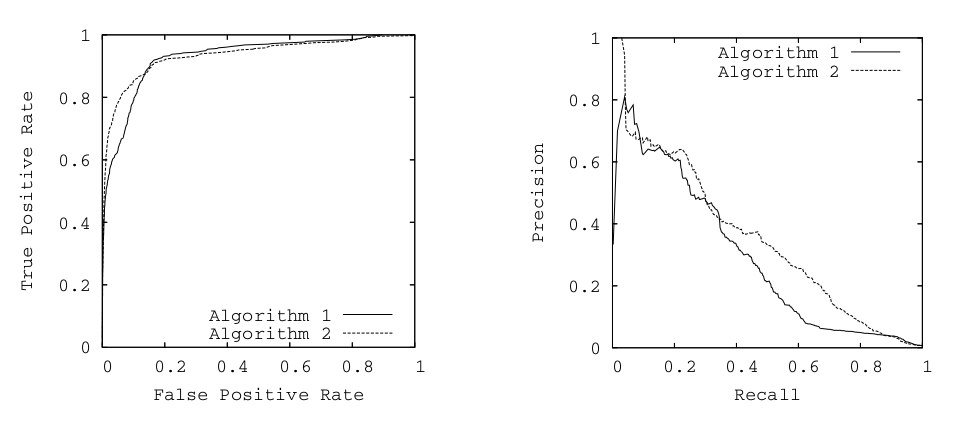
\includegraphics[width = 0.83\textwidth]{plots/AUCandPRAUC.png}
	\caption[Sample ROC and PR curves]{A sample receiver operating characteristic curve (left) and precision-recall curve (right). Each algorithm is evaluated on different thresholds and the points produced are used to obtain the curves. Image courtesy of~\cite{Davis2006}}
	\label{fig:AUCandPRAUC}
\end{figure}

For unbalanced data sets, ``using the classifiers produced by standard machine learning algorithms without adjusting the output threshold may well be a critical mistake''~\cite{Provost2000}. It is preferable to use metrics that consider all possible thresholds (AUC or PRAUC) or simpler metrics ($F_1$ score or G-mean) with a threshold obtained via a validation set. The metric used for model selection influences its characteristics and behaviour, hence, it should be chosen carefully: we favor the use of PRAUC over AUC as well as $F_1$ score over G-mean because they concentrate in the positive class (disease) that is more interesting and harder to predict. Furthermore, PRAUC has been shown to have better properties than AUC in unbalanced data sets~\cite{Davis2006}. % In general, results for all these metrics.
We introduce metrics tailored to image segmentation models in Sec.~\ref{sec:Segmentation}.
%F1 better represents a more balanced tradeoff  (an small change in precision is corresponded with a small change in recall) than AUC where an small change in specificity can be corresponded with a big change in sensitivity.

\begin{comment} Discussion of why G-mean over F1
(Not sure about this) As a rule of thumb, using G-mean will generate models that predict more positives given that the sensitivity will greatly improve and specificity will only slightly decrease. Using $F_1$ score, the model will predict less positives as that will improve precision but only slightly decrease sensitivity. 
5 here say PRAUc is better for unbalanced classes

Why G-means? Because it is more important to obtain a low error in specificity than in precision, i .e, would you prefer a 90% in specificity or a 90% in precision?. 90% in specificity means that 10% of actual negatives (10 persons) were told they have no cancer although they actually had cancer, meanwhile 10% of expected positives(a small number, maybe 1) was said he has cancer although he doesn{t. First is worse.

Using G-mean i will predict more positives, no matter what. My sensitivity is going to vastly improve and the specificity will only decrease a little, but the precision is gonna take a hit. Because if I predict less positives sensitivity is gonna go down, specificity is gonna go up (as I add more true negatives) but just a little and precision  would go up (but it wouldn't matter for g-mean).

Using F1 I'll probably predict less positives, sensitivity is going to go slightly down, and precision is going to go up, specificity doesn{t matter but it will decrease a little. Or I'll probably predcit as many poositives as needed. It focuses more on the positive class.

Other diagonal, the algorithm will learn negatives pretty well, so the one that predicts less positives(f1) probably isn{t learning much (it is predicting all negative).
\end{comment}

%We point out that this section introduces basic concepts in machine learning but leaves aside many practical details. Content and notation is based on materials from Stanford's Machine Learning course~\cite{Ng2014}.


\section{Artificial Neural Networks}
\label{sec:ANNs}
\emph{Artificial neural networks} or simply \emph{neural networks} are one of the most popular nonlinear classifiers. Although initially inspired in the way biological neurons integrate information~\cite{McCulloch1943, Widrow1960, Rosenblatt1962}, they evolved to specialize in nonlinear modelling at the expense of biological adherence~\cite{Rumelhart1986}.% We discuss here multilayer feedforward neural networks, the name should become obvious after a few paragraphs.

\emph{Multilayer feedforward neural networks} are composed of $L$ layers of \emph{neurons}, the computation units.% Each unit is connected to every unit in the previous and next layer.
%[[; units in a layer are|, ] [fully] connected to [every] units in|. Each layer is fully connected to] the previous and next layer (except for [units in] the first and last layer
The first layer, called the \emph{input layer}, has $s^{(1)} = n$ units and receives the feature vector $x \in \mathbb{R}^n$ while the last layer or \emph{output layer} has $s^{(L)} = K$ units corresponding to the $K$ possible classes. Every other layer is called a \emph{hidden layer} (Fig.~\ref{fig:NeuralNetwork}). The neural network receives an input $x \in \mathbb{R}^n$, processes it layer by layer and outputs a vector $h_\Theta(x) \in \mathbb{R}^K$, where $h_\Theta(x)_k$ is the predicted (unnormalized log) probability that $x$ belongs to class $k$. Each unit performs a computation on the output from units in the previous layer and transmits the result to units in the next layer through their connections. Furthermore, every connection has a \emph{weight} $w$ that is learned in the training phase, i.e, the weights are the parameters $\Theta$ of the model. A neural network is \emph{shallow} or \emph{deep} according to its number of layers or \emph{depth}: networks with one or more hidden layers are considered deep.

\begin{figure}[h]
	\centering
	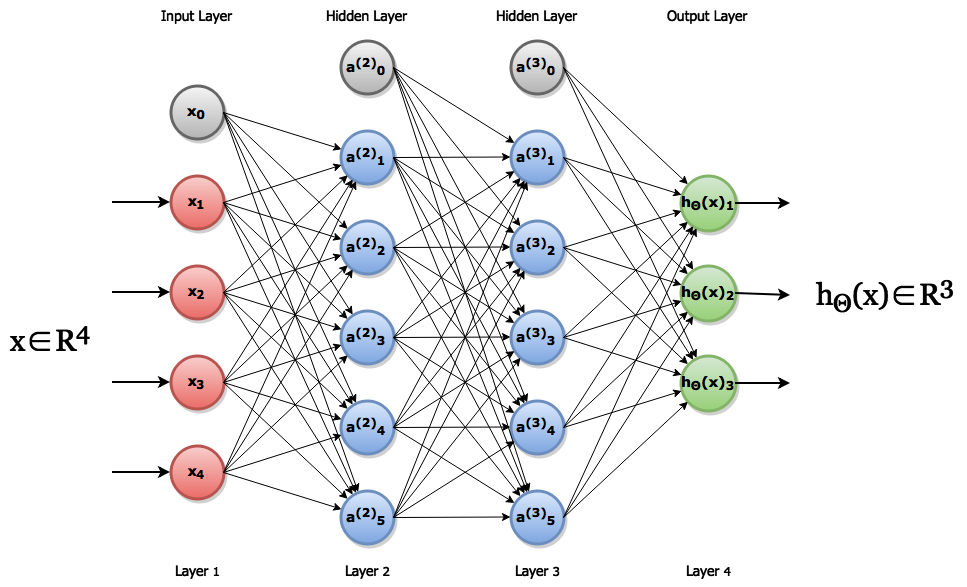
\includegraphics[width = 0.93\textwidth]{plots/neuralNetwork.png}
	\caption[An artificial neural network]{A small neural network: input layer with 4 units (red), two hidden layers of 5 units (blue) and output layer of 3 units (green). Bias units appear in gray. It approximates a function $h_\Theta(x): \mathbb{R}^4 \to \mathbb{R}^3$, i.e., it classifies an input vector $x \in \mathbb{R}^4$ into 3 possible classes.}
	\label{fig:NeuralNetwork}
\end{figure}

A unit computes a function of the form:
\begin{equation}
	a^{(l)}_i = g \left(\sum_{j=0}^{s^{(l-1)}} \Theta^{(l-1)}_{ij}a_j^{(l-1)}\right) \text{ for $l= 2,\dots,L-1$ and $i = 1,\dots,s^{(l)}$}
	\label{eq:NeuronActivation}
\end{equation}
where $a^{(l)}_i$ is the \emph{activation} or output of unit $i$ in layer $l$;
$g(\cdot)$ is an \emph{activation function} (defined below);
$s^{(l)}$ is the number of units in layer $l$;
$a^{(u)}_0 = 1$, for all $u = 1, \ldots, L-1$ (defined below);
$a^{(1)}_v = x_v$ for all $v = 1, \ldots, n$ i.e., the activation of the input layer is the input $x$;
$a^{(L)}_i = \sum_{j=0}^{s^{(L-1)}} \Theta^{(L-1)}_{ij}a_j^{(L-1)}$ for all $i = 1,\dots,s^{(L)}$ i.e., $g(\cdot)$ is omitted in the output layer
and $\Theta^{(l)} \in \mathbb{R}^{s^{l+1} \times s^{l}} $ is the matrix of weights connecting layer $l$ to $l+1$. Equation~\ref{eq:NeuronActivation} seems convoluted but it simply defines the activation of a unit as the weighted linear combination of the activations of units in the previous layer passed through a nonlinear function $g(\cdot)$. 

Each layer (except for the output layer) includes a \emph{bias unit} that outputs 1 regardless of its input ($a^{(1)}_0 = 1$, $a^{(2)}_0 = 1$, etc) allowing units in the next layer to learn a parameter $\Theta_{i 0}$ to account for its own predisposition to activate.
%~\footnote{This mechanism is rather technical and depends on the activation function.} |More technichally, they allow the y intercept of ... to be different thna 0 giving us more expressive power. 
Bias units are included in the vectors $a^{(l)}$, hence, the sumation in Equation~\ref{eq:NeuronActivation} starts at 0 instead of 1.

\begin{comment}
The activation function $g(\cdot)$ is usually a \emph{logistic sigmoid function}:
\begin{equation}
	g(z) = \frac{1}{1+ e^{-z}}
\end{equation}
The sigmoid function has range [0,1] and is differentiable with respect to $z$. Because of this characteristics it is used to represent probabilities in the logistic regression classifier. \emph{Logistic regression} for binary classification models the probability that $x \in \mathbb{R}^n$ belongs to the positive class as $g(w^Tx)$ and estimates the parameters $w \in \mathbb{R}^n$ during training. Any input whose output $g(w^Tx)$ is greater than $0.5$ is classified as positive, otherwise it is classified as negative. The sigmoid function equals $0.5$ when $w^Tx = 0$, thus, the decision boundary of a logistic regression classifier is $w^Tx = 0$, which is a linear function. 

However, the sigmoid function, per se, is not linear on its input $z$. Therefore, each unit in a neural network with sigmoid activation functions outputs a nonlinear activation $g(z)$ which in turn is received by units in the next layer, linearly recombined with the activation of other units and passed again through a sigmoid function; these operations are repeated until the input reaches the output layer. As a result, the function calculated by units in the output layer $h_\Theta(x)$ will be highly nonlinear on the original input $x$. This is the reason why neural networks can model functions which are highly nonlinear and why increasing the number of layers in a neural network increases the predictive power of the model. By the same token, it may be insightful to think of each unit in a neural network as a feature detector (via logistic regression): units in the first hidden layer are trained to activate when simple features are found on the input, units on the second hidden layer activate when a combination of these simple features is present on the input and so on. Thus, the network will learn to detect the most relevant features for the classification task and as the number of units increases, it learns ever more complex features (granted that there is enough training data).
\end{comment}

The activation function $g(\cdot)$ is usually a \emph{rectified linear unit} or \emph{ReLU}:
\begin{equation}
	g(z) = \max(0,z)
\end{equation}
This nonlinear function and its derivative ($1_{z>0}$) are computed easily and, unlike sigmoid or tanh activation functions, are inmune to vanishing and exploding gradients. Besides, it greatly accelerates convergence of gradient descent~\cite{Krizhevsky2012} and is currently the recommended activation function for deep neural networks~\cite{Karpathy2016}.

The vector of activations in the output layer $a^{(L)} \in \mathbb{R}^{s^{(L)}}$, called a \emph{score vector}, is the predicted (unnormalized log) probabilities $h_\Theta(x) \in \mathbb{R}^K$ that example $x$ belongs to class $k \in K$. We can exponentiate each of these values and normalize them to obtain a probability distribution over the possible classes $K$ ($p(x) \in [0..1]^K$); this improves interpretability and preserves original predictions.

Every unit produces a nonlinear activation $g(z)$ that is received by units in the next layer, linearly recombined with the activation of other units and passed again through the nonlinear function $g(z)$; these operations repeat until the processed input reaches the output layer. As a result, the network computes a function $h_\Theta(x)$ that is highly nonlinear on the original input $x$. This explains why neural networks are able to model complex functions and why increasing the number of layers increases its expressive power. It may be insightful to think of each unit as a feature detector: in the first hidden layer, units learn to detect simple features of the input, in the second hidden layer, units activate when a distinct combination of the simple features is found and so on. Thus, the network learns to recognize the most relevant features of the input learning more complex features as the number of units increases.

The \emph{softmax} loss function for a multiclass neural network classifier is defined as:
\begin{equation}
	L(\Theta) = -\frac{1}{m} \sum_{i=1}^m \log \left ( \frac{ e^{h_\Theta(x^{(i)})_{y^{(i)}}} }{ \sum_{j=1}^K e^{ h_\Theta (x^{(i)})_j} } \right )
\end{equation}
where $m$ is the number of examples in the training set, $h_\Theta(x)$ is the score vector, $K$ is the number of classes and $(x^{(i)},y^{(i)})$ is the $i^{th}$ example. $L(\Theta)$ is differentiable with respect to $\Theta$ but non-convex, nonetheless, gradient descent usually converges to a good estimate of $\Theta$~\cite{Ng2014}. \emph{Error backpropagation}~\cite{Linnainmaa1970, Werbos1974}, an algorithm to calculate the derivatives of the loss function with respect to $\Theta$, computes error terms in the output layer and backpropagates them layer by layer using the chain rule of calculus.

%Deep neural networks are suceptible to overfitting because they need to estimate many parameters. 
Because many parameters need to be estimated, deep neural networks are susceptible to overfitting. The simplest approach to overcome this is using regularization. Regularization for neural networks is done by performing gradient descent on the regularized loss function presented in Equation~\ref{eq:ANNRegularizedLossFunction}
\begin{equation}
	L(\Theta) = -\frac{1}{m} \sum_{i=1}^m \log \left ( \frac{ e^{h_\Theta(x^{(i)})_{y^{(i)}}} }{ \sum_{j=1}^K e^{ h_\Theta (x^{(i)})_j} } \right ) + \frac{\lambda}{2m}\sum_{l=1}^{L-1}\sum_{i=1}^{s^{(l)}}\sum_{j=1}^{s^{(l+1)}} \left(\Theta^{(l)}_{ij}\right)^2
	\label{eq:ANNRegularizedLossFunction}
\end{equation}

\emph{Dropout}~\cite{Srivastava2014} is another popular method to prevent overfitting. Each training iteration, dropout samples a different network architecture from the original network and updates only a subset of the values in $\Theta$; a unit (and its connections) is retained with some probability $p$ (usually 0.5-1), and gradient descent works on this sampled network (Fig.~\ref{fig:Dropout}). During testing all units are active but their activations are scaled by $p$ to match their expected output ($p a^{(l)}_i + (1-p) 0$). This is interpreted as training many models (with shared weights) and averaging their results at test time.

\begin{figure}[h]
	\centering
	\begin{subfigure}{0.3\textwidth}
                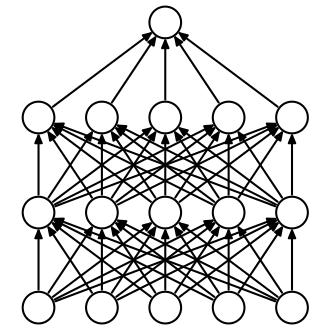
\includegraphics[width=\textwidth]{plots/dropout1.png}
		\caption{Standard neural network}
        \end{subfigure}
	~
	\begin{subfigure}{0.3\textwidth}
                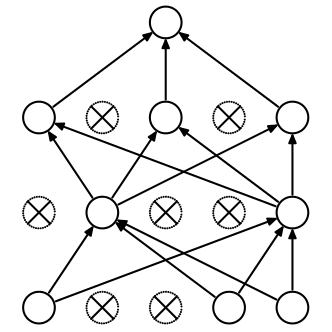
\includegraphics[width=\textwidth]{plots/dropout2.png}
		\caption{After applying dropout}
        \end{subfigure}
	\caption[Example of Dropout]{Dropout applied to a simple neural network. Crossed units are dropped. Image courtesy of~\cite{Srivastava2014}.}
	\label{fig:Dropout}
\end{figure}


\section{Convolutional Networks}
\label{sec:ConvNets}
\emph{Convolutional networks}, also \emph{ConvNets} or \emph{CNNs}, were first inspired by the way the human visual cortex proccesses information~\cite{Fukushima1980} but, as regular neural networks, have evolved to favor practical performance over biological accuracy. LeCun et al. used a convolutional network to achieve good classification performance on the MNIST data set of handwritten digits~\cite{LeCun1989, LeCun1998}, the first successful application of modern convolutional networks. Recently, Krizhevsky et al. used  them to achieve state-of-the-art performance on the ImageNet Large-Scale Visual Recognition Challenge~\cite{Krizhevsky2012}, an image classification and object localization challenge with 1000 categories~\cite{Russakovsky2014}. Thanks to various advances (maxpooling, ReLU activations, weight initialization, GPU training, efficient backpropagation, etc.), convolutional networks have become one of the most popular methods for image classification tasks and (along with recursive neural networks) an emblem of deep learning.

In this section we show the standard features and training of current convolutional networks. Section~\ref{subsec:PracticalDL} gives some practical advice for choosing hyperparameters and training deep architectures. For an in depth review of convolutional networks, see \cite{Karpathy2015}. For a complete overview of the history and state of deep learning, see \cite{Schmidhuber2015}.

Convolutional networks map raw image pixels to a score vector $h_\Theta(x) \in \mathbb{R}^K$ representing the distribution of (unnormalized log) probabilities over the $K$ classes. We could use a regular neural network (presented in Section~\ref{subsec:ANNs}) to do this but the amount of learnable parameters (the weights) becomes very big. For instance, a small color image of size $100\times100$ with 3 color channels (RGB) will require $30\,000$ units in the input layer and each unit in the second layer will therefore have $30\,000$ weights to learn. This is impractical not only because it will require a lot of data and training time but because the loss function has very many local minima and thus it is harder to optimize.

Convolutional networks reduce the number of connections between layers and the number of parameters to learn. Convolutional layers are \emph{sparsely connected}, i.e., a unit is only connected to a small subset of the units in the previous layer. Furthermore, they are \emph{locally connected}, i.e., units are connected considering their position on the original image. The architecture of a convolutional network also imposes \emph{weight sharing} between units in the same layer, i.e., different units are forced to share the same weights (this determines filters and feature maps, defined below). \emph{Pooling} is a subsampling mechanism that reduces the spatial scale and makes the computations invariant to local translation. All these features reduce computation and improve the classification performance of convolutional networks; they are produced by the way convolutional networks are defined, which we explain below.

Each layer is composed of a set of \emph{feature maps}, 2-dimensional grids of unit activations~($\mathbb{R}^{h\times w}$), arranged into a 3-dimensional matrix ($\mathbb{R}^{h\times w \times d}$). We use the third dimension to put together all feature maps. One could unfold a 3-dimensional volume to form a single column of unit activations as in regular neural networks but seeing them as a volume makes the definitions easier. The input layer is a 3-dimensional matrix ($\mathbb{R}^{h\times w \times c}$) that holds the input image of size $w\times h$ with $c$ color channels ($c = 1$ for grayscale images or $c = 3$ for RGB). The output layer is a volume of size $R^{1\times 1 \times K}$ where each feature map is just one activation ($R^{1\times 1}$) representing the final score. The network receives an image $x$ as an input volume that is transformed layer by layer into new volumes (whose dimensions could be different from the previous one) until it reaches the output layer of size $h(x) = R^{1\times 1 \times K}$. See Fig.~\ref{fig:ConvNetVolumes} for an illustration. We describe the transformations next.
\begin{figure}[h]
	\centering
	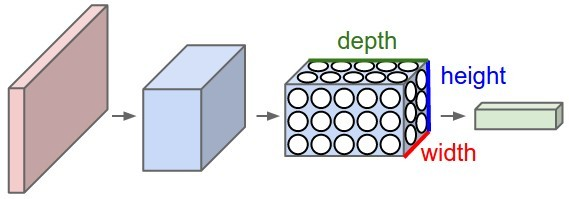
\includegraphics[width = 0.7\textwidth]{plots/convNetVolumes.jpeg}
	\caption[Convolutional network visualization]{A simple representation of the transformations of the input computed by a convolutional network. Input layer is shown in pink, hidden layers are shown in blue and output layer is shown in green. The third layer has 5 feature maps of size $2\times3$. Notice that the width is listed first by convention. Image courtesy of~\cite{Karpathy2015}.}
	\label{fig:ConvNetVolumes}
\end{figure}

Four types of layers are commonly used: convolutional layer, ReLU layer, pooling layer and fully connected layer; all of which compute a differentiable function on its input and combine to form a convolutional network architecture.

\paragraph{Convolutional layer} Convolutional layers are the heart of convolutional networks. They are build by learnable filters that are applied to the volume in the previous layer. A \emph{filter} is a matrix of weights that has a small spatial size (width and height) but goes across all feature maps of the volume (the third dimension). For instance, a $3\times 3$ filter to be applied in a volume with 10 feature maps will have 90 parameters ($\mathbb{R}^{3\times3\times10}$). See Figure~\ref{fig:ConvLayer} for an example. Each feature map in this layer is obtained by sliding a filter across the spatial dimensions (width and height) of the previous volume computing the dot product (a weighted sum) between the filter and the input~\footnote{Each filter has also a bias term added to the sum.}. All values in a single feature map are computed using the same filter. If we think of the feature map as a grid of units we can see that every unit is connected with only a small local subset of the units in the previous layer and that all units in the map share the same weights. 

At each convolutional layer, many feature maps are computed (each with its own filter) and stacked together to form the volume in the layer. We can think of each filter as looking for an specific feature on the input and each feature map as the probabilities of that feature in each position.

We choose various hyperparameters for this layer: the filter size, the stride (the number of places to shift the filter at each step), the amount of zero padding around the image and the number of feature maps. These define the shape of the resulting volume; the first three are usually chosen to preserve the spatial size of the previous volume, the number of feature maps depends on the amount of features we want to learn.
\begin{figure}[h]
	\centering
	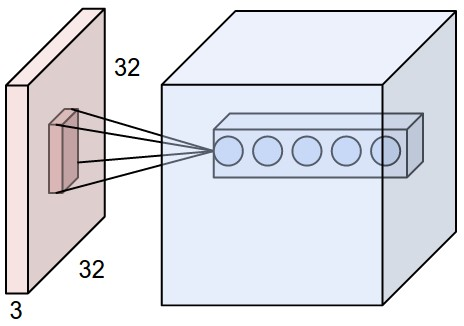
\includegraphics[width = 0.4\textwidth]{plots/convLayer.jpeg}
	\caption[Example of a filter in a convolutional layer]{Example of a filter applied to a volume ($\mathbb{R}^{32\times 32\times 3}$) to obtain the values shown in the blue volume. The filter comprises all 3 feature maps of the input volume. We compute 5 feature maps as shown by the 5 units in the blue volume. For a complete convolution this filter will have to slide across the input volume. All units in the same feature map share the same filter but units in different feature maps do not, even though they can be connected to the same local region of the input. Image courtesy of~\cite{Karpathy2015}.}
	\label{fig:ConvLayer}
\end{figure}

\paragraph{ReLU layer} This layer receives an input volume and performs an elementwise ReLU activation function to it, i.e, each value $z$ in the volume is passed through the nonlinearity $\max(0,z)$. It preserves the dimensions of the volume and has no learnable parameters, although the activation function may be considered a hyperparameter. Usually, a ReLU layer (or any other activation function) follows a convolutional layer, for this reason it is sometimes considered part of the convolutional layer. We separate them for clarity.

\paragraph{Pooling layer} The pooling layer subsamples the volume on the spatial dimensions reducing the size of the feature maps but keeping the number fixed. Standard max pooling slides a fixed size windows (normally $2\times2$) along each feature map with stride 2 (it is, without overlapping) and selects the maximum element on that space. This will reduce each dimension of the feature map by half, thus reducing the total number of activations by 75\%, e.g., a $4\times4$ feature map gets subsampled to size $2\times 2$ where each value is the maximum activation on each of the four quadrants of the original feature map. Contrary to convolution, subsampling is applied to each feature map separately. A popular variant of max pooling uses $3\times 3$ windows with stride 2, allowing for some overlapping.

\paragraph{Fully connected layer} We use one or more fully connected layers at the end of the network to compute the final score vector. Feature maps in this layer have size $1 \times 1$ resulting in a row volume or alternatively a row vector of values. Each feature map in this layer is fully connected to all units in the previous volume and outputs a dot product between the input and the connection weights, which are the parameters to be learned during training. The output layer of a convolutional network is always a fully connected layer with as many feature maps as classes. We interpret the scores of the output layer similar to those of regular neural networks as the (unnormalized log) probability of $x$ belonging to class $k$. Lastly, notice that a fully connected layer can be simulated by a convolutional layer with the same number of feature maps and filter size $w\times h$ where $w$ and $h$ are the spatial dimensions of the previos volume, i.e., filters that comprise the entire volume.

\bigskip
Convolutional layers (plus ReLUs) compute features on the input while pooling layers shrinken the volume before passing to the fully connected layers that act as a regular neural network classifier on the obtained features. The standard convolutional network architecture can be represented textually as:
\begin{verbatim}
       INPUT -> [[CONV -> RELU]*N -> POOL?]*M -> [FC -> RELU]*K -> FC
\end{verbatim}
where \texttt{*N} indicates that the layers are repeated \texttt{N} times, \texttt{?} indicates that the layer is optional and \texttt{N,M,K >= 0}. We can use this template to construct ever more flexible models from a linear classifier \texttt{INPUT -> FC} (\texttt{N,M,K = 0}) to a regular neural network \texttt{INPUT -> [FC -> RELU]+ -> FC} (\texttt{N,M = 0}, \texttt{K > 0}) to a convolutional network \texttt{INPUT -> [[CONV -> RELU]+ -> POOL?]+ -> [FC -> RELU]* -> FC} (\texttt{N,M > 0}, \texttt{K >= 0}). For instance, a typical deep convolutional network could be:
\begin{verbatim}
        INPUT -> [[CONV -> RELU]*2 -> POOL]*3 -> [FC -> RELU]*2 -> FC
\end{verbatim}
This network receives an input volume (the image) computes two sets of convolution plus ReLUs before pooling and repeats this pattern three times followed by fully connected layers plus ReLUs which are repeated twice and the output layer that reports the final classification scores. Although there is no standard way of counting the number of layers, we usually ignore the ReLU and pooling layers as they have no learnable parameters. Therefore, our example has 10 layers (21 in total), which is a good depth for big data sets. Practical recommendations on building architectures is offered in the Section~\ref{subsec:PracticalDL}.

Figure~\ref{fig:ConvNetExample} shows an example of a convolutional network with its different kind of layers. The image is taken from a simulation accesible at \url{cs231n.stanford.edu}.

\begin{figure}[h]
	\centering
	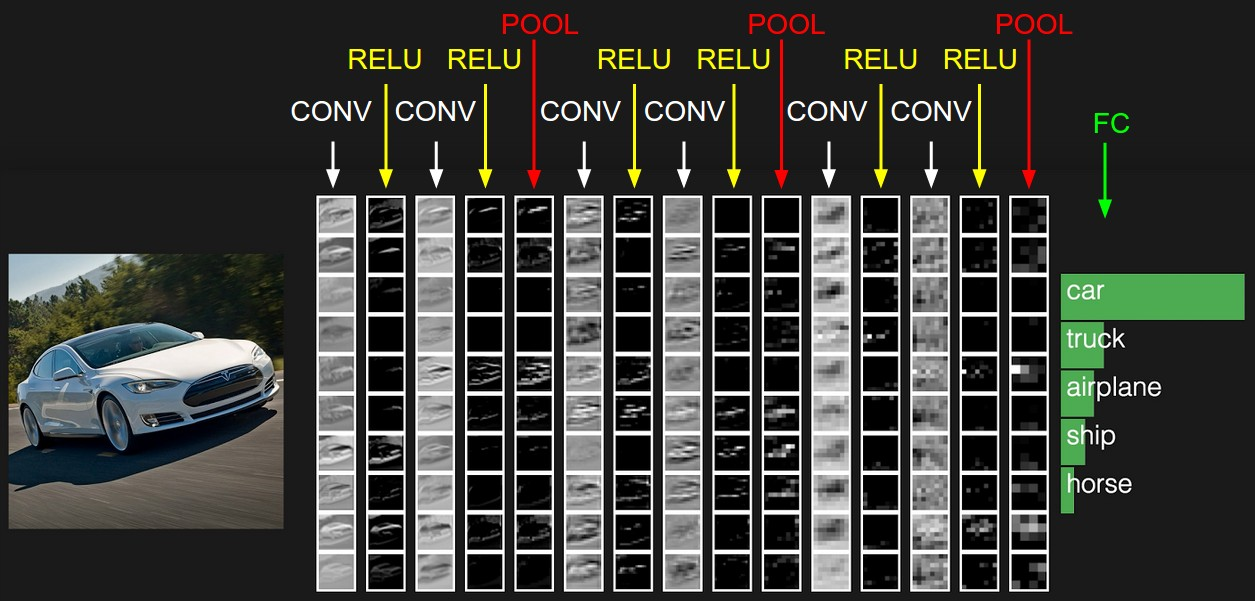
\includegraphics[width = 0.85\textwidth]{plots/convNetExample.jpeg}
	\caption[Example of a convolutional network in action]{Example of a convolutional network with architecture \texttt{INPUT -> [[CONV -> RELU]*2 -> POOL]*3 -> FC}. The input image has size $32\times 32$. Each hidden layer uses 10 feature maps (shown as columns). Although the spatial size of the feature maps looks constant in the image, each pooling layer reduces its dimensions by half (the feature maps of the final pooling layer have size $4\times 4$). We show the final scores only for the five most probable classes. Image courtesy of~\cite{Karpathy2015}.}
	\label{fig:ConvNetExample}
\end{figure}

Recently, simpler convolutional network architectures have emerged. The All Convolutional Net~\cite{Springenberg2014} is a network formed solely by convolutional layers: we replace pooling layers by convolutional layers with larger strides and fully connected layers as explained above. This greatly increases the number of parameters to be learn, therefore it is unsuitable for small data sets.

Converting the fully connected layers to convolutional layers has another advantage: we can use a convolutional network trained on small images to classify bigger images. By the way convolutional layers are defined when we use a bigger image as input the entire convolutional network will slide across the image and be applied to different portions of the image generating a score vector for each of them. Therefore, instead of having a single score for each class we will have an entire matrix of scores (for each position where the convolutional network was applied). Then, we can average over all scores per class to obtain a single score vector for the bigger image. Furthermore, we can control the stride of the convolution to choose how the convolutional network is slided across the big image.
For instance, if we train a convolutional network with images of size $32\times 32$ that via pooling get reduced to feature maps of size $4\times 4$ in turn passed to the (converted) fully connected layers to obtain a score vector, then when using a $96\times 96$ image as input to the same convolutional network it will get reduced to feature maps of size $12 \times 12$ and the fully connected layers will output a matrix of scores of size $9\times 9$ (for each class), i.e, it slides the $4\times 4$ fully connected layers across the $12\times 12$ feature maps. Averaging each score matrix we obtain the final scores for the big image. We could have also  set a stride of 4 in the first (converted) fully connected layer to get score matrices of size $3\times 3$ for each 9 non-overlapping $32\times 32$ partitions of the original image. It works exactly as if we applied the convolutional network to the original image at a stride of 32 but does all computations in just one pass. This way we can reuse a pretrained network to classify images of bigger size. 

\emph{Transfer learning} is a related method where we train a convolutional network on images from a specific domain and later use it to extract features on images from a different domain. It could also be used as a initialized network which is fine tuned with examples of the new domain.

The loss function for a multiclass convolutional neural network is similar to that for a regular neural network (Equation~\ref{eq:ANNRegularizedLossFunction}) except that now the convolutional network defines the vector score $h_\Theta(x)$.
\begin{equation}
	J(\Theta) = -\frac{1}{m} \sum_{i=1}^m \log \left ( \frac{ e^{h_\Theta(x^{(i)})_{y^{(i)}}} }{ \sum_{j=1}^K e^{ h_\Theta (x^{(i)})_j} } \right ) + \frac{\lambda}{2m}\sum_{l=1}^{L-1}\sum_{i=1}^{s^{(l)}}\sum_{j=1}^{s^{(l+1)}} \left(\Theta^{(l)}_{ij}\right)^2
	\label{eq:ConvNetLossFunction}
\end{equation}
Furthermore, this loss function is still differentiable with respect to $\Theta$ and thus we can train the entire network via gradient descent. We use backpropagation to calculate the gradients of the loss function.


\section{Image Segmentation}
\label{sec:Segmentation}
%\emph{Image segmentation} is the process of [labelling|colloring|classifying] each pixel in [an|the] image [as belonging to |with the label from] an object present depending on conforming corresponding (Fig~\ref{fig:imageSegmentation}).
\emph{Image segmentation} is the task of labelling each pixel in an image according to the object to which it belongs (Fig~\ref{fig:imageSegmentation}).
We can segment an image by training a classifier on small patches, sliding it across bigger images to obtain per-pixel predictions and assigning each pixel to its highest predicted class.
%~\footnote{For classification, we average score vectors across pixels to obtain a single vector for the bigger image.}
\begin{figure}[h]
	\centering
	\begin{subfigure}{0.26\textwidth}
                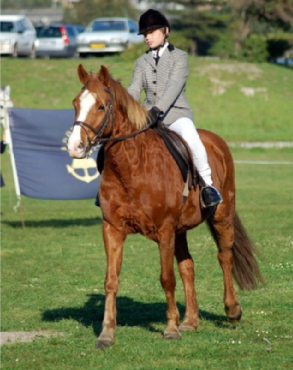
\includegraphics[width=\textwidth]{plots/segmentationImage.png}
		\caption{Original image}
        \end{subfigure}
	~
	\begin{subfigure}{0.26\textwidth}
                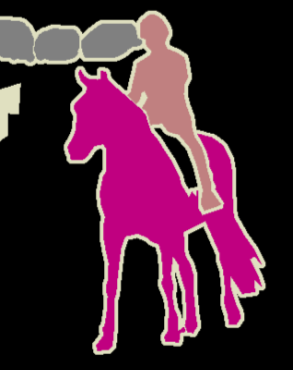
\includegraphics[width=\textwidth]{plots/segmentationTruth.png}
		\caption{Segmentation}
        \end{subfigure}
	\caption[Segmentation of an image]{Segmentation of an image with five classes. Image courtesy of~\cite{Long2015}}
	\label{fig:imageSegmentation}
\end{figure}

Convolutional networks are specially apt for image segmentation: we can transform each fully connected layer into a convolutional layer by padding the input volume to preserve spatial dimensions~\footnote{Padding by $\lfloor (f_s-1)/2\rfloor$ where $f_s$ is the filter size.} creating a network that is able to segment images of any size, albeit, due to subsampling in the pooling layers, it produces a coarse segmentation that needs to be upsampled to match the size of the original image.
%Adding zero-padding to each fully connected layer~\footnote{As with convolutional layers, padding the input volume by $\lfloor (f_s-1)/2\rfloor$ where $f_s$ is the filter size.} creates a convolutional network that is able to segment images of any size, albeit, due to subsampling in the pooling layers, produces a coarse segmentation that needs to be upsampled to match the size of the original image.
%Convolutional networks automatically behave this way when presented with a bigger image than those used for training, albeit, due to subsampling in the pooling layers, they produce a coarse segmentation that needs to be upsampled to match the size of the original image.
For instance, a convolutional network trained with $32\times 32$ images and two pooling layers (that reduce the input by a factor of 4) acts as a $32 \times 32$ filter with stride 4 so for a $256 \times 256$ image it will produce a $64 \times 64$ segmentation that needs to be upsampled by a factor of 4 to recover the original dimensions.
\begin{comment}
We could also set a stride of 4 in the first (converted) fully connected layer to get score matrices of size $3\times 3$ for each 9 non-overlapping $32\times 32$ partitions of the original image. It works exactly as if we applied the convolutional network to the original image at a stride of 32 but does all computations in just one pass.
if we augment the stride of the firs fully connected layer we can compute coarser segmentations or
\end{comment}
%For training, the loss function sums the loss over all pixels; to account for the mismatch between the output of the network and the ground truth image (labels), which has the dimensions of the original image, we downsample the ground truth image or append an upsampling layer at the end of the network. This layer computes a differentiable function either fixed such as bilinear interpolation or learned such as a linear mapping; adding this upsampling layer forms a \emph{fully convolutional network}~\cite{Long2015}.
To account for the difference in size between the output of the network and the label image---the ground truth segmentation\textemdash, we downsample the label image or append an upsampling layer at the end of the network~\cite{Long2015}; the additional layer computes a differentiable function either fixed such as bilinear interpolation or learned such as a linear mapping.
%; this forms a \emph{fully convolutional network}~\cite{Long2015}.
%Setting the loss function to sum the loss over all pixels completes the modifications needed.
%Subsampling, however, afects the granularity of the predicted segmentation.
Alternatively, we could remove pooling layers and use \emph{dilated convolutions}, filters with spaces between any two values (Fig.~\ref{fig:DilatedConvolutions}), thus enlarging the receptive field of the filter as pooling would do but keeping the spatial dimensions of the volume and the number of parameters fixed~\cite{Yu2016}.
\begin{figure}[h]
	\centering
	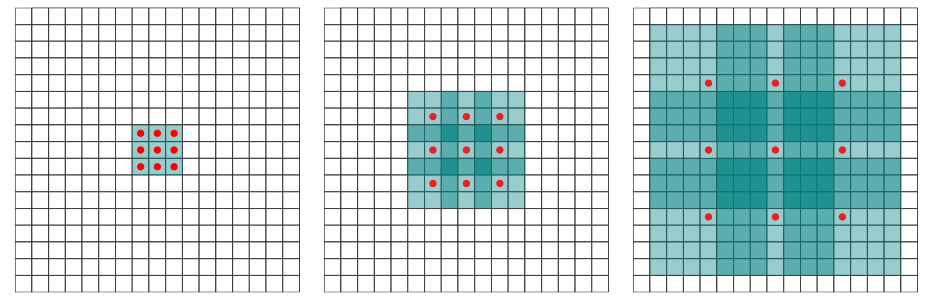
\includegraphics[width=0.8\textwidth]{plots/dilatedConv.png}
	\caption[Example of dilated convolutions]{Example of a $3\times3$ convolutional filter at increasing dilations: zero, two and four. The spatial dimensions of the input volume are represented as a black grid, red dots signal the places where the filter is applied and the green shadows represent the effective receptive field of the filter. Courtesy of~\cite{Yu2016}.}
	\label{fig:DilatedConvolutions}
\end{figure}

Lastly, the loss function sums the loss over all pixels so the network performs a single gradient update after one example segmentation. Convolutional networks transform image segmentation into an end-to-end, learnable task.

% Results are evaluated [using|with] the metrics [defined |introduced|used] [for|in] [classification|section] [computed|applied] pixelwise..
% [To evaluate results|For evaluation,|] we [compute|use|measure] [the average of|image-wise|] [classification|evaluation] metrics [for each|per|in each] [image|segmentation] and average [over all [of them| segmentations| images]]; for instance, [pixel] accuracy [measures|is] the (average) proportion of correctly classified pixels in [one|an] [image.
%To evaluate results, we use classification metrics (Sec.~\ref{sec:Classification}) averaged over all images; for instance, pixel accuracy is the average proportion of correctly classified pixels per image. Other metrics are calculated similarly.
%To evaluate results, we measure a classification metric per segmentation and average its result over all segmentations; for instance, pixel accuracy measures the (expected) proportion of correctly classified pixels in a segmentation.
%We use \emph{pixel accuracy}, the proportion of correctly classified pixels in a segmentation, to evaluate results. Evaluation metrics, including pixel accuracy, are the average value of a classification metric (Sec.~\ref{sec:Classification}) measured on segmentations produced for the test set. 
%To evaluate results, we compute the average value of a classification metric (Sec.~\ref{sec:Classification}) measured on segmentations produced for the test (or validation) set. \emph{Pixel accuracy}, for instance, estimates the (expected) proportion of correctly classified pixels in a segmentation.
%Evaluation metrics are the average value of a classification metric (Sec.~\ref{sec:Classification}) measured on segmentations produced for the test (or validation) set. \emph{Pixel accuracy}, for instance, estimates the (expected) proportion of correctly classified pixels in a segmentation.
%To evaluate the model, we measure a classification metric (Sec.~\ref{sec:Classification}) on segmentations of images in the test set and average the results;
To evaluate the model, we evaluate each segmentation using standard metrics (Sec.~\ref{sec:Classification}) and average over all test images. \emph{Pixel accuracy}, for instance, is the average proportion of correctly classified pixels in an image.
%[Other metrics are calculated| We calculate other metrics] [similarly|in a similar fashion]. 
Another popular metric, \emph{intersection over union} or \emph{IOU}, is calculated for a single segmentation as $TP/(TP+FP+FN)$ (Tab.~\ref{tab:ConfusionMatrix}).
%IOU = DC/(2-DC) (DC: Dice coefficient)
%DC = 2IOU/(IOU+1)
In medical diagnosis, the \emph{free-response operating curve} or {FROC curve} evaluates a radiologist or CAD system at localizing lesions: for varying thresholds, the FROC curve plots the sensitivity of the system (proportion of lesions correctly localized) versus the number of false positives commited per image. We can compare between models using their sensitivity at a fixed number of false positives per image, for instance, sensitivity at 1 FP/image.

If we are interested in a particular class, e.g. object vs. background, we present a single score map showing its probability distribution across every position in the image. We can refine this map using gaussian smoothing, cluster-based thresholding and conditional random fields among other techniques. Finally, to produce a segmentation we threshold the post-processed map at some specific value, which can be chosen using a validation set.
 

\section{Practical Deep Learning}
\label{sec:PracticalDL}
In this section we collect some recommendations for constructing convolutional networks as well as efficiently training deep neural networks. These are intended to be specific to this project but most will also be useful in similar projects.
% Some of these details are taken care by the software(either as a defualt or optional feature) and some are qyuite new and need to be taken care manually. 

\paragraph{Image preprocessing} Some standard processing for images.
\begin{itemize}
	\item Images are cropped to contain only the relevant parts of the image, denoised, enhanced and optionally downsampled to maintain the input size fixed and manageable.

	\item Each image feature (the raw pixels) is zero centered by substracting its mean across all training images. Normalization scales the already zero-centered features to range from $[-1 \dots 1]$ by dividing them by its standard deviations. Feature normalization is not striclty neccesary but still customary~\cite{Karpathy2015}.

	\item The test data should not be used to calculate any statistic used to preprocess the training data. Furthermore, these same statistics (calculated from the training data) should be used when normalizing the test data~\cite{Karpathy2015}.
\end{itemize}

\paragraph{Convolutional network architecture}
We offer some guidelines for designing convolutional network architectures and some standard values for various hyperparameters.

\begin{itemize}
	\item It is always better to select a complex network architecture which is flexible enough to model the data and manage overfitting with regularization rather than an architecture which is not powerful enough to model the data~\cite{Ng2014, Krizhevsky2012}. 

	\item Although, theoretically, neural networks with a single hidden layer are universal approximators provided they have enough units ($\mathcal{O}(2^n)$ where $n$ is the size of the input), in practice, deeper architectures produce better results using less units overall. This insight holds for convolutional networks~\cite{Bengio2014}.

	\item As a rule of thumb for big data sets, use 8-20 layers (not counting pooling or ReLU layers). For small data sets, use less layers or transfer learning. ``You should use as big of a neural network as your computational budget allows, and use other regularization techniques to control overfitting.''~\cite{Karpathy2015}

	\item Use the number of parameters rather than the number of layers or units as a measure of the architecture's complexity.

	\item Use 2-3 \texttt{CONV -> RELU} pairs before pooling (N above)~\cite{Karpathy2015}. Pooling is a destructive operation and having two convolutional layers together allows them to pick up more complex features.

	\item Use 1-5 \texttt{[CONV -> RELU]+ -> POOL} blocks (M above). This number depends on the complexity of the features expected in the data and the computational resources available. In a way, this regulates how much representational power will the architecture have. It also decides how much the volume is subsampled.

	\item Use less than 3 \texttt{FC -> RELU} pairs before the output layer (K above)~\cite{Karpathy2015}. When the volume arrives to the fully connected layers it has shrinken enough and using more fully connected layers risks overfitting.

	\item The number of feature maps per convolutional layer is set according to the expected number of features. This is similar to the number of units in a regular neural network. A common pattern is to start with a small amount of feature maps and increase them layer by layer~\cite{Simonyan2014}. %The reasoning is that at higher layers there are more complex features to learn and moreover as the feature maps become smaller (via pooling) it is computationally feasible to have more of them.

	\item The number of feature maps per fully connected layer, or equivalently the number of units per fully connected layer, decreases from the number of units in the last convolutional layer (the number of units in each feature map times the number of feature maps) to the number of classes. For instance, having a convolutional network with two fully connected layers and 10 possible classes if the last convolutional layer produces a volume of size $8 \times 8 \times 512$ (8192 units), the first fully connected layer could have size $1 \times 1 \times 2048$ and the second (output) layer $1\times 1\times 10$.

	\item Use $3\times 3$ filters with stride 1 and zero-padding 1 or $5 \times 5$ filters with stride 1 and zero-padding 2. This preserves the spatial dimensions of the volume and works better in practice~\cite{Springenberg2014}. When training on big images, the first convolutional layer uses bigger filters~\cite{Karpathy2015}.
	
	\item Use $2\times2$ pooling with stride 2. Both this pooling and the overlapping version presented in Section~\ref{subsec:ConvNets} produce similar results. Pooling divides the spatial dimensions of the volume in half~\cite{Krizhevsky2012}.
%krizhevsky says overlapping is slightly better. so does dieleman but it slows thing down.
	\item Use square input images (width = height) with dimensions divisible by 2. The dimensions should be divisible by 2 at least as many times as the number of pooling layers in the network.

	\item Convert fully connected layers into convolutional layers.
\end{itemize}



\paragraph{Hyperparameter search}
We deal here with choosing hyperparameters other than those of the network architecture.

\begin{itemize}

	\item Use a single sufficiently large validation set (20-30\%) rather than cross validation~\cite{Bengio2014}. For small data sets, cross validation can give better estimates and is preferred~\cite{Ng2014}.

	\item Use random search rather than grid search. Random search draws each parameter from a value distribution rather than a set of predefined values.~\cite{Bergstra2012}

	\item Train each parameter combination for 1-2 epochs to narrow the search space. Later, train for more epochs on the refined ranges. Full convergence is not needed to make a decision on the hyperparameters~\cite{Karpathy2015}.

	%\item Use a different validation set if you need to run the hyperparameter search for new parameters. :: Because the old validation set is already good for the hyperparameters chosen, we want to choose good hyperparameters in general not only in that validation set.

	\item Hyperparameters related to the convolutional architecture, e.g., number of layers, number of feature maps, filter sizes, etc., are set manually (as explained above) rather than using a validation set.
% M,N,K, filter size, stride and padding in each convolutional layer, feature maps and units in CONV/FC layers, pooling

	\item There are several hyperparameters to set: initial learning rate $\alpha$, learning rate decay schedule, regularization strength $\lambda$, momentum $\mu$, probability of keeping a unit active in dropout $p$, mini-batch size and type of image preprocessing.

	\item Theoretically we could fit all the hyperparameters using a validation set but in practice it is computationally unfeasible and could result in overfitting the hyperparameters to the validation data~\cite{Cawley2010}.

	\item Set $\alpha$, $\lambda$ and optionally the type of preprocessing using a validation set. Other hyperparameters can be set to a sensible default. 
%The learning rate schedule and training epochs are set using heuristics. 

	\item The learning rate $\alpha$ is ``the single most important hyperparameter and one should always make sure that it has been tuned''~\cite{Bengio2012}. It ranges from $10^{-6}$ to $10^{0}$. Use a log scale to draw new values ($\alpha = 10^{unif(-6, 0)}$ where $unif(a,b)$ is the continous uniform distribution)~\cite{Karpathy2015}.
%0.01: Bengio, 2012 says that the optimal learning rate is close to the highest learning rate that does not cause divergence.

	\item The regularization strength $\lambda$ is usually data (and loss function) dependant. It ranges from $10^{-3}$ to $10^4$. Search in log scale ($\lambda = 10^{unif(-3, 4)}$).
%1

	\item If the best values for a hyperparameter are found in the limit of the range, explore further.~\cite{Bengio2012}.

	\item Use standard image enhancements. If there are no standard methods, use the validation set to choose from the options.

	\item Halve the learning rate every time the validation error stops improving. To obtain a fixed number of epochs, train the network (with the obtained hyperparameters) and observe when the validation error stops decreasing~\cite{Krizhevsky2012}.

	\item Use $\mu=0.9$. When using a validation set try values in \{0.5, 0.9, 0.95, 0.99\}~\cite{Karpathy2015}.

	\item Use 0.9-1 probability $p$ of retaining a unit in the input layer, 0.65-0.85 in the first 2-4 convolutional layers and 0.5 in the last convolutional layers and all fully connected layers~\cite{Srivastava2014}. Less dropout is used on the first layers because they have less parameters~\cite{Karpathy2015}.
% Maybe don't use dropout in the input layer, because putting a zero there has a meaning(black), maybe the advantage of dropout in cinvolutional layers is just that it adds noise to the input.

	\item Use mini-batch size of 64 or 32. A larger batch size requires more training time. It affects training time more than test performance~\cite{Bengio2012}.

\end{itemize}



\paragraph{Training}
Some general tips for efficiently training convolutional networks with million of parameters and very big data sets. Using these algorithms for small networks may be somewhat excessive but it will not hurt the performance.

\begin{itemize}
	\item Randomize the order of the trainig examples before training. As we are using an stochastic estimator of the gradient this ensures the examples in each batch are sampled independently. Shuffling the examples after each epoch could also speed convergence~\cite{Bengio2012}.

	\item To estimate the number of examples needed to train a convolutional network divide the total number of learnable parameters by 25-100 (assuming some data augmentation). Some groups have been able to learn up to 40M parameters from as little as 60K training examples~\cite{Dieleman2015, Springenberg2014}.

	\item Weight initialization is very important for a proper convergence of the network. The current recommendation for ReLU units is to initialize each weight as a value drawn from a gaussian distribution $\mathcal{N}(\mu = 0, \sigma = \sqrt{2/n_{in}})$ where $n_{in}$ is the fan-in of the unit, i.e., the number of inputs to the unit. Specifically, each filter weight could be initialized as \texttt{w = randn()*sqrt(2/nIn)} where \texttt{randn()} returns a value drawn from a standard normal distribution and \texttt{nIn} is the number of connections to this filter (9 for a $3\times 3$ filter, for example). Weights for units in the fully connected layer follow the same formula. Biases can be initialized likewise or to zero~\cite{He2015}.

	\item Use mini-batches to compute the gradient. Using the entire training set to compute the gradient of the loss function takes a big amount of computation and points to the steepest descent direction locally but may not be the right direction if the update step is large. Using mini-batches allows us to make more updates, more frequently which results in faster convergence and better test results~\cite{Bengio2012}.

	\item Use Nesterov's Accelerated Gradient (NAG) to update the weights. It is a modified version of gradient descent which has shown to work slightly better for certain architectures~\cite{Bengio2012b}. Stochastic Gradient Descent with Momentum (SGD+Momentum) is also a viable option~\cite{Karpathy2015}.
% May need to crossvalidate the momentum if using NAG 

	\item Use dropout as a complement to $l_2$-norm regularization. Dropout usually improves results but it may slow network convergence~\cite{Krizhevsky2012}.

	\item Store the network parameters regularly during training. Once per epoch should be enough but it depends on the number of parameters and size of the data. This allows you to come back to different versions of the network and select the one with the best overall validation/test error or one with some special characteristics~\cite{Bengio2014}.

	\item Stop the training process when the validation or test error has not improved since the last learning rate reduction. At this point gradient descent may not have converged but the validation error has and will start to increase (overfit)~\cite{Bengio2012}.

	\item Use the validation or test error to select the best parameters for the network from those stored~\cite{Bengio2014}. 

	\item If you use the test set to refine a model, shuffle the entire data set and choose a diferent training and test set for the new model. Otherwise, you run the risk of overfitting to the test set~\cite{Ng2014}.
\end{itemize}



\paragraph{Sanity checks}
Some simple checks to make sure the training is working properly.
\begin{itemize}
	\item After weight initialization, the network should predict similar scores for each class (uniform probability) and have a loss function (without regularization) equal to $-\log(1/K)$. You can check this by running a test on a small set of examples. Adding regularization should increase the loss~\cite{Karpathy2015}.

	\item If you implement back propagation manually or believe it may not be working properly you can run a gradient check. Gradient checks compare the analytic gradient produced by backpropagation with a numerical gradient produced by a finite difference approximation~\cite{Karpathy2015}.

	\item Train the network with a very small subset of data (20 examples, for instance) and make sure it produces zero loss (without regularization). If it cannot overfit a tiny subset of examples the model is too simple~\cite{Ng2014}.

	\item During training, the training loss should always decrease or only slightly increase. Otherwise, gradient descent may not be working properly either because of an implementation error or poorly tuned hyperparamters (high learning rate, low momentum)~\cite{Karpathy2015}.

	\item Monitor the training and validation loss during training to identify overfitting and underfitting. Underfitting is characterized for a high training loss, overfitting is characterized for a big gap between training and validation (or test) loss~\cite{Ng2014}.
\end{itemize}

\paragraph{Data augmentation}
One of the easiest ways to reduce overfitting in image data is to generate additional examples from the original data by applying some simple label-preserving transformations. Data augmentation allows the network to see different views of the same object thus enabling it to identify features that do not depend on the invariance introduced by the transformations. 
For instance, if we present it with images of a book on different rotations, we expect it to learn to identify a book no matter its position.

\begin{itemize}
	\item There are many transformations one can apply: rotations, translations, horizontal and vertical reflections, crops (sample patches of the original image), zooms, etc. For color images, adding some noise to (jittering) the colors is also a valid transformation.
% Dieleman galaxies didn't like jittering or scales and crops
% Lo liked rotation and horizontal flipping

	\item Exploit the invariances you expect in the data set. For instance, galaxies are rotation invariant given that in space there is no up or down~\cite{Dieleman2015} but trees are not as it is rare to see an upside down tree.

	\item When combining different transformations in the same image be careful to preserve the original label. An overly modified image may lose its meaning. 

	\item Most transformations are affine in the geometric plane and can be combined into a single one. If you plan to apply various transformations to the same image, applying a single affine transformation is faster and reduces information loss~\cite{Dieleman2015}.

	\item Generate the augmented images during training. This saves storage and can be performed alongside the training~\cite{Krizhevsky2012}.

	\item Data augmentation can also be used at test time by presenting the network with various versions of the same image and averaging its predictions~\cite{Krizhevsky2012}. 
	
\end{itemize}

% Need some sources for this section. I've read it all around.
\paragraph{Unbalanced data}
Having very few examples of one class compared to the rest is common in practice. We offer here some advice to deal with unbalanced classes using standard convolutional networks. We note that there is no accepted way to manage this problem.
\begin{itemize}
	\item For a binary classifier, if the positive class is the rare class use PRAUC as a performance metric. If you are reporting the $F_1$ score, you should select an appropiate threshold using a validation set~\cite{Davis2006}.

	\item If using PRAUC or selecting the threshold with a validation set is impractical, a simple adjustment is to divide the predicted probabilities by their corresponding class priors and to renormalize the values.

	\item For multiclass classification, use the macro-averaged $F_1$ score, an average of $F_1$ scores per class, with validated thresholds~\cite{Ozgur2005}. A multiclass PRAUC also exists but it is not as easy to interpret.

	\item As the threshold setting does not affect training it can be fitted independently of other hyperparameters once the network has already been trained. If fitting more than one, consider each one as a separate hyperparameter and use random search to find the best combination.

	\item One of the preferred methods to learn with unbalanced data sets is to use a modified loss function which gives a higher weight to errors in the rare class so that during training errors in the rare class will produce higher learning in the network parameters. Specific knowledge of the domain is required to estimate the cost of each class of error.

	\item Oversampling and undersampling, repeating the examples of the rare class or discarding some examples from the dominant class, are discouraged because they either not add information or throw away some of it.

	\item Replicating rare examples (oversampling) is useful when the examples are very scarce and the classifier simply does not have enough data to learn. This could be achieved by balancing the classes on each mini-batch via stratified sampling or by augmenting the rare class more than the dominant class during data augmentation.

	\item Data augmentation differs from data replication in that it only tries to enrich the data set with invariant images but actually leaves the proportion of classes unchanged.
\end{itemize}

\paragraph{All convolutional networks}
The research community has been moving towards discarding the pooling layers and using all convolutional networks. This can be interpreted as letting the network learn the pooling operation. We offer a couple of guidelines for implementing all convolutional networks.  
\begin{itemize}
	\item Replace each pooling layer with a convolutional layer with as many feature maps as in the previous layer and filter size $2\times 2$ with stride $2$ for normal pooling or $3\times 3$ with stride $2$ for overlapping pooling~\cite{Springenberg2014}. 

	\item For small data sets pooling layers also work as a regularizer because they reduce the number of learnable parameters and replacing them with convolutional layers may not be convenient~\cite{Karpathy2015}.
\end{itemize}

\paragraph{Transfer learning}
When we have a small data set we could use a pretrained convolutional network either as a feature extractor for the new examples or to provide initializations for the new convolutional network, this is called transfer learning. We offer some tips for using a pretrained model specifically for mammographic images.

\begin{itemize}
	\item Using a convolutional network pretrained in natural images, such as the ImageNet database, CIFAR-10, CIFAR-100, etc., may not work for mammographic images because features useful for one kind of classification are not very useful for the other. Nonetheless, given that features become more specific at higher layers, we could discard the higher layers of the network and use only the cropped network~\cite{Karpathy2015}.
 
	\item Depending on the amount of data that we have we could: (1) add some fully connected layers on top of the pretrained network and train only these new layers, (2) add some convoutional and fully connected layers and train these new layers or (3) add convolutional and/or fully connected layers and train the entire network~\cite{Karpathy2015}.

	\item When training on a pretrained model or fine-tuning use an smaller learning rate than when training a network from scratch. Using a small learning rate assures that we do not disturb very much the already good network parameters.~\cite{Karpathy2015}.
\end{itemize}

\paragraph{Software}A short description of four of the most popular packages for deep learning. They are pretty similar in capabilities and availability (open-source).

\begin{itemize}
	\item Caffe~\cite{Jia2014}: Caffe is an already mature deep learning framework developed in C++/CUDA by the Berkeley Vision and Learning Center (BVLC) and community contributors. It offers a command line, Python and Matlab interface, reference models and tutorials and very fast code with easy GPU activation.
	\item Torch7~\cite{Collobert2011}: Torch is a scientific computing framework developed in C/Lua/CUDA at the IDIAP Research Institute. It offers n-dimensional arrays (tensors), automatic differentiation, a command line and Lua interface, GPU support and easy building of complex neural network architectures.
	\item Theano~\cite{Bergstra2010, Bastien2012}: Theano is a Python library developed in Python/CUDA at the University of Montreal. It is tightly integrated with NumPy, performs symbolic automatic differentiation and uses the GPU to efficiently evaluate mathematical expressions involving multi dimensional arrays.
	\item Cuda-ConvNet2~\cite{Krizhevsky2014}: Cuda-ConvNet2 is a highly optimized convolutional network library developed in C++/CUDA by Alex Krizhevsky. It offers different off-the-shelf configurations for convolutional networks, a command line interface and multi-GPU training.
\end{itemize}

\bigskip

Lastly, we acknowledge that mammographic data is fairly different to that used in common object recognition tasks, for instance, labelling may not be as sharp or correct, images come in different sizes and ratios, image quality varies, the object to recognize may be very small in relation to the image, object localization may be a requirement, etc. and therefore some of the advice given above may prove counterproductive. When possible, design decisions should be based on the data and results obtained until that point.

%We plan to start with a simple convolutional architecture and add some of the well tested features first and other possible features later to obtain an optimized model which will be trained and tes.

%Deep Learning (Bengio Lecture): (https://www.youtube.com/watch?v=JuimBuvEWBg)


\section{Breast Cancer}
\label{sec:BreastCancer}
\emph{Cancer} is an umbrella term for a group of diseases caused by abnormal cell growth in different parts of the body. The accumulation of extra cells usually forms a mass of tissue called a \emph{tumor}. Tumors can be benign or malignant: \emph{benign tumors} are noncancerous, lack the ability to invade surrounding tissue and will not regrow if removed from the body;  malignant or \emph{cancerous tumors} are harmful, can invade nearby organs and tissues (\emph{invasive cancer}), can spread to other parts of the body (\emph{metastasis}) and will sometimes regrow when removed~\cite{NCI2012}.

\emph{Breast cancer} forms in tissues of the breast. The two most common types of breast cancer are \emph{ductal carcinoma} and \emph{lobular carcinoma}, which start in the breast ducts and lobules, respectively (Fig.~\ref{fig:BreastAnatomy}). Breast cancer \emph{incidence rate}, the number of new cases in a specified population during a year, is the highest of any cancer among American women. Its \emph{mortality rate}, the number of deaths during a year, is also one of the highest of any cancer~\cite{Howlader2014}.

\begin{figure}[h]
	\centering
	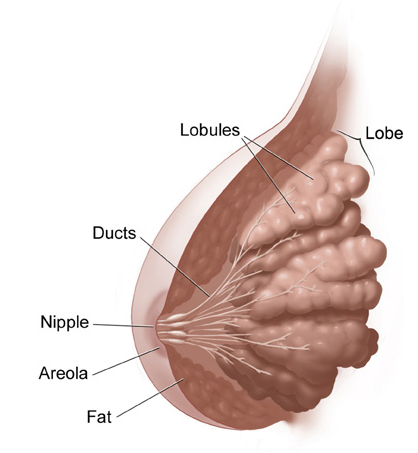
\includegraphics[width = 0.34\textwidth]{plots/breastAnatomy.png}
	\caption[Anatomy of the female breast]{Anatomy of the female breast. Image courtesy of~\cite{NCI2012}.}
	\label{fig:BreastAnatomy}
\end{figure}

The \emph{cancer stage} depends on the size of the tumor and whether the cancer cells have spread to neighboring tissue or other parts of the body. It is expressed as a Roman numeral ranging from 0 through IV; stage I cancer is considered \emph{early-stage breast cancer} and stage IV cancer is considered \emph{advanced}. Stage 0 describes non-invasive breast cancers, also known as \emph{carcinoma in situ}. Stage I, II and III describe invasive breast cancer, i.e., cancer has invaded normal, surrounding breast tissue. Stage IV is used to describe metastatic cancer, i.e., it has spread beyond nearby tissue to other organs of the body.

\subsection{Mammograms}
%\subsubsection{Mammograms}
A \emph{mammogram} is an x-ray image of the breast. Radiologists use \emph{screening mammograms} (normally composed of two mammograms of each breast) to check for breast cancer signs on women who lack symptoms of the disease. If an abnormality is found, a \emph{diagnostic mammogram} is ordered; these are detailed x-ray pictures of the suspicious region~\cite{NCI2014}. A standard mammogram is shown in Figure~\ref{fig:normalMammogram}.

\begin{figure}[h]
	\centering
	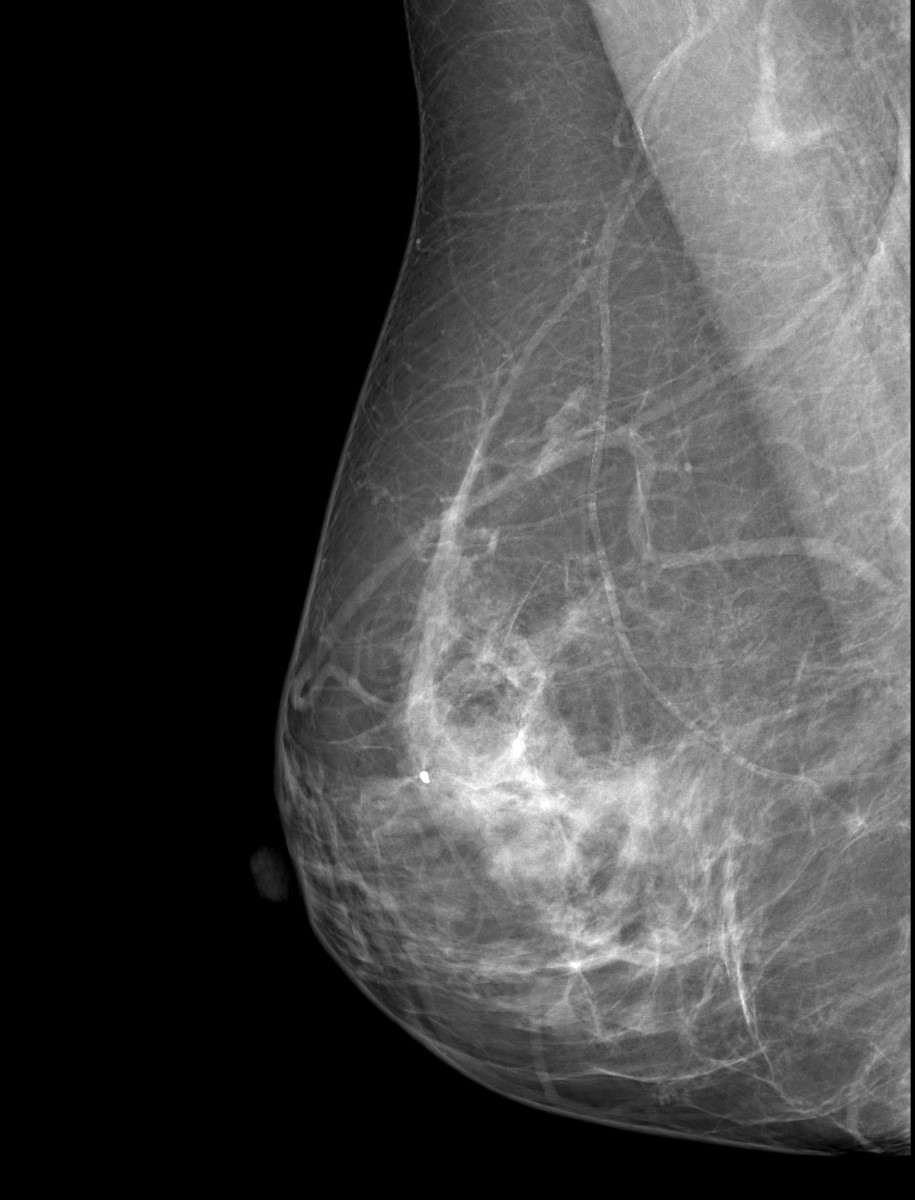
\includegraphics[width = 0.25\textwidth]{plots/normalMammogram.jpg}
	\caption[A digital mammogram]{A standard mammogram.}
	\label{fig:normalMammogram}
\end{figure}

Having a screening mammogram in a regular basis is the most effective method for detecting breast cancer early; around 85\% of breast cancers can be detected in a screening mammogram~\cite{BCSC2013}. Nevertheless, screening mammograms have many limitations: a high false positive rate, overtreatment in Stage 0 cancer, false negative results for women with high breast density, radiation exposure and physical and psychological discomfort~\cite{NCI2014}.

Radiologists look primarily for microcalcifications and breast masses. \emph{Microcalcifications} are tiny deposits of calcium in the breast tissue that can be a sign of early breast cancer if found in clusters with irregular layout and shapes (Fig.~\ref{fig:breastCancerSigns}). \emph{Breast masses} or breast lumps are a variety of things: fluid-filled cysts, fibric tissues, noncancerous or cancerous tumors, among others. A mass can be a sign of breast cancer if it has an irregular shape and poorly defined margins (Fig.~\ref{fig:breastCancerSigns}). Radiologists will also consider the breast density of the patient when reading a mammogram given that high breast density is linked to a higher risk of breast cancer~\cite{ACS2014}.
\begin{comment} My classification
Lesion
	Mass = Lump(This is palpable)
		Malignant = Cancerous
			Tumors
		Benign = Noncancerous
			Tumors
			Cysts
			Fibrosis/Fibroadenoma
	Microcalcifications (benign or malignant)

Tumors are abnormal growths of cells, cysts ae filled with fluid and fibrosis are "firmness in the connective tissues". Lesion is anything suspicious in a mammogram
Detection: Find lesions (malignant or benign)
Diagnosis: Find malignant lesions
\end{comment}

\begin{figure}[h]
	\centering
	\begin{subfigure}{0.24\textwidth}
                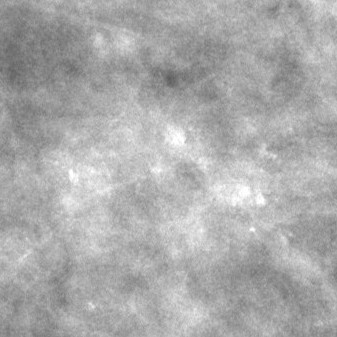
\includegraphics[width=\textwidth]{plots/breastMicrocalcification.jpg}
        \end{subfigure}
	~
	\begin{subfigure}{0.24\textwidth}
                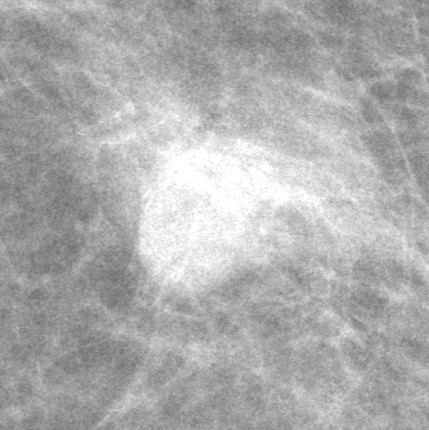
\includegraphics[width=\textwidth]{plots/breastMass.jpg}
        \end{subfigure}
	\caption[Signs of possible breast cancer]{Signs of possible breast cancer in a mammogram. Left: A cluster of microcalcifications in an irregular layout. Right: A poorly defined breast mass.}
	\label{fig:breastCancerSigns}
\end{figure}

%Conventional mammography uses film to record x-ray images of the breast. \emph{Digital mammography}, on the other hand, uses digital receptors that convert x-rays into electrical signals and stores the image electronically. 
Conventional mammography records mammograms in film; \emph{digital mammography}, on the other hand, converts x-rays into electrical signals and stores images electronically.
Digital mammograms offer a clearer picture of the breast and ease manipulation and sharing between health care providers.
% However, researchers still debate whether [[its|their] use over| they] [surpass| improve on|outperform|[offers|have] an advantage over|are more effective than|benefit] film mammograms [in|for] [identifying breast cancer|breast cancer detection].
Although researchers still debate whether they offer an advantage over film mammograms~\cite{Kerlikowske2011, Pisano2008, Skaane2007}, digital mammography has become standard in breast cancer screening. Figure~\ref{fig:normalMammogram} is, in fact, a digital mammogram.
\emph{Digital tomosynthesis} is a new technology that produces three-dimensional x-ray images of the breast and improves the efficacy of mammograms in certain escenarios~\cite{Tagliafico2016}.%http://jco.ascopubs.org/content/early/2016/03/07/JCO.2015.63.4147.abstract
%is expected to improve the efficacy of mammograms. Studies comparing the two techniques have not yet been published~\cite{NCI2014}.

\emph{Computer-aided detection (CAD)} systems assist radiologists during screening signaling suspicious areas and displaying relevant information. Detection or CADe looks for any type of lesion while diagnosis or CADx focuses on malignant lesions. Whether their use improves accuracy has been challenged~\cite{Lehman2015}.

% option: Delete this, downgrade mammograms to subsubsection and add the bcdr info in the solution/data set/database part. Maybe also leave the first paragraph in here as part of mammograms subsection, only change it to say "Mammography databases are important"
% option: do not add anything
\subsection{Mammographic databases}
%Databases are essential to mammographic image analysis;
%annotated
Researchers use data from previous patients---mammograms, segmentations and clinical features\textemdash to train and evaluate their models. 
%Databases offer pixel-wise labelled mammograms, lesions are segmented by expert radiologists.
%For this purpose, lesions are manually segmented to produce pixel-wise labels.
\emph{Contrast resolution}, the number of gray values per pixel, and \emph{spatial resolution}, breast area per pixel, dictate the quality of a digital mammogram: 12-bit images ($2^{12} = 4048$ gray values) with pixel size of at most 0.1mm are prefered. Many publicly available databases, including those described below, satisfy these conditions.

The Digital Database for Screening Mammography (DDSM)~\cite{Heath2001} is the most popular database used for CAD development. It is composed of around 10.5K digitized film mammograms from 2620 patients. Mammograms are either 12-bit or 16-bit images with 0.05 mm spatial resolution. Lesion segmentations are provided along with its type, assesment, subtlety and malignancy.%Patient data is also provided.
%Type is mass, microcalcification, assesment (1-5) in BIRADs, subtlety(1-5) and 

The BancoWeb database~\cite{Nepomuceno2011} consists of around 1.5K digitized film mammograms from 300 Brazilian patients. Mammograms are 12-bit images with 0.075 or 0.15 mm pixel size. Although few lesions are segmented, this repository may be useful to assess performance in Latin American patients. Its current state is unknown.

Lastly, the Breast Cancer Digital Repository (BCDR-DM)~\cite{Moura2013a, Moura2013b} consists of around 1.2K digital mammograms from 237 patients. Mammograms are 8-bit images with 0.07mm spatial resolution.
Lesion segmentations are provided as well as their assesment, hand-crafted texture and shape features and relevant clinical data.
%It provides lesion segmentations and assesments, hand-crafted texture and shape features and relevant clinical data

\begin{comment}
Another small digital mammogram repository is called INbreast~\cite{Moreira2012}. It consists of 410 digital mammograms from 115 patients. Each mammogram is a 14-bit image with 0.7 mm spatial resolution. Lesion boundaries are accurately marked and its information is also included. This could be used in conjunction with the BCDR-DM repository.

Finally,~\cite{Zheng2012} used a private repository of around 6.5K digital mammograms obtained from 1120 patients. Specifics of contrast and spatial resolution are not provided but they are most probably good enough. Lesions are marked (with a circle) on the mammograms and lesion and patient information is provided. Even though this is a private repository of the University of Pittsburgh, if needed, we could ask them for access to it. This may not be plausible given the complications of sharing personal (granted anonymized) information and the size of the database.
\end{comment}

This section was written using information from the National Cancer Institute. We recommend to visit its website (\url{www.cancer.gov}) for further details.


\section{Convolutional Networks in Breast Cancer Research}
\label{sec:BreastCancerConvNets}
Traditional CAD systems for breast cancer detection (CADe) and diagnosis (CADx) are normally composed of various succesive stages: preprocessing and image enhancement, segmentation of suspicious regions, feature extraction from the segemented image patches, optionally feature selection and region classification using machine learning methods. \cite{Tang2009} offers a good review of the current state of traditional CAD systems. Here we focus on the previous application of convolutional networks for breast cancer detection and diagnosis in mammographic images.

As explained in Section~\ref{subsec:BreastCancer} there are two main signs of breast cancer: breast masses and clustered microcalcifications, however, their presence does not necessarily imply cancer because they could be benign lesions. We refer as detection to the task of classifying a lesion as present or absent in the image no matter its malignancy, for instance, classifying an image patch as either clustered microcalcifications or normal tissue, while we talk of diagnosis when classifying a lesion as either benign or malignant~\footnote{Images without lesions are considered benign.}.

%There are mainly two groups who have worked on convolutional network aapplied to breast cancer: one from the Department of Radiology of the University of Michigan and one from the Department of Radiology of Georgetown University.
\paragraph{Overview}
The only work using convolutional networks to detect masses was presented in~\cite{Sahiner1996}. Although the network produced competitive results, research focused more on feature-based classifiers, such as regular neural networks, that produced better results using expert knowledge and advanced image techniques. Around the same time,~\cite{Lo1995} presented the first use of convolutional networks to detect individual microcalcifications. This work was followed up by~\cite{Gurcan2002} who looked to select an optimal convolutional network architecture for individual microcalcification detection. This optimized network was used in two CADe systems for clustered microcalcifications: one for film mammography~\cite{Gurcan2002} and one for digital mammography~\cite{Ge2006}. Both systems have a similar layout consisting of preprocessing, image enhancement, segmentation of potential microcalcifications, false positive reduction, regional clustering and false positive reduction of clusters. The convolutional network plays a relatively small role as an individual microcalcification classifier during the first false positive reduction stage. Lastly, recently an unpublished report~\cite{Agarwal2015} uses a convolutional network for the diagnosis of breast lesions obtaining average results.

In summary, convolutional networks have been sporadically used for breast cancer detection and diagnosis but have only played a minor role. Other than the most recent application, researchers have used very small networks (2 or 3 layers, $<$10K parameters) withouth any recent advancement (ReLUs, pooling layers, regularization, GPU computation) trained on very little data to classify image patches that were preselected using advanced image techniques. For instance, convolutional networks have only been used to detect individual microcalcifications but not clusters of microcalcifications and although they have been used to detect breast masses, using a larger network could probably improve those results. They have not been used for any type of breast cancer diagnosis either.

In the following sections we expand on the work mentioned above. We present a thorough summary of the most important articles organized by topic.

\begin{comment}
Separated in blocks:
	1. Initial mass: Sahiran 1996 (michigan)
	2. Intial microcalc detection: Lo 1995- Lo 1998 (georgetown/both)
	3. Optimal architecture for microcalc: Gurcan 2000-Gurcan 2002 (michigan)
	4. CAD for microcalcification in FFDM. Ge 2007 (CAD for masses didn't use Convnets, used LDA and rule-based classifiers). (michigan)
	5. Unpublished Stanford convnet: Agarwal 2015 (stanford)
\end{comment}

\subsubsection{Detection of masses}
%******************************** Wei1995 *******************************************
% Wei, Datong, Sahiner, Berkman, Chan, Heang-Ping, Petrick, Nicholas. Detection of masses on mammograms using a convolution neural network (1995) ICASSP, IEEE International Conference on Acoustics, Speech and Signal Processing - Proceedings, 5, pp. 3483-3486.
% Pretty much the same as Sahiner1996 but smaller and simpler.
To the best of the author knowledge, the first attempt to use convolutional networks for breast cancer is reported in "Detection of masses on mammograms using a convolution neural network"~\cite{Wei1995}. This 4-page article was later expanded in~\cite{Sahiner1996}.

%******************************** Sahiner1996 **************************************
% Sahiner, B., Chan, H.-P., Petrick, N., Wei, D., Helvie, M.A., Adler, D.D., Goodsitt, M.M. Classification of mass and normal breast tissue: A convolution neural network classifier with spatial domain and texture images (1996) IEEE Transactions on Medical Imaging, 15 (5), pp. 598-610. 
\begin{comment}
- detection of tumors
- uses mass to mean benign or malign tumors (growths of cell with no purpose) and normal tissue is other masses (cysts, liquids, no mass at all, etc)
- 168 mammograms: 168 positive classes, 504 negative classes
- 0.87 AUC, 0.9 sensitivity, 0.69 specificity
- texture "contains useful information that can be used to effectively distinguish masses from normal tissue." Not sure 'bout this
- one output sigmoid
- GD+momentum, adaptive learning rates,  early stopping
- manually extracted ROI's
- "The average size (length of the long axis) of the masses, as estimated by the radiologists, was 12.2 mm., and the standard deviation of the mass size was 4.5
mm." i could use a 2-2.5 cm filter.
- digitized mammograms (not digital)
- For each mamogram, 4 ROIs extracted (a tumor, fatty tissue, dense tissue nad mixed dense/fatty tissue)
- each pixel 0.1 mm
- 256 pixels by 256 pixels initial image (2.56 cm by 2.56 cm)
- background reduction (averaging a 2 by 2 box with an average of 4 cardianl boxes). 
- (Because they didn't have the power) nonoverlapping average pooling (where the avg function is applied instead of the max function) with 16 x 16 filters (rsulting in 16 by 16 image patches) and 8 by 8 filters (resulting in 32 by 32 image patches)
- 8 rotations(0,90,180,270 and flipped). Used all to calculate a single output for training, so all 8 will contribute a single number. Output obtained as average among all of them.
 
- Experiment with single input image:
	single hidden layer network with variable feature maps and kernel size.
	Best results with kernel size 10 for 16 and 20 for 32.
	small grid search(needed to test more values).
	0.83 AUC
- GLDS texture features: contrast, angular second moment, enlropy and mean. Calculated at different subregions of the original 256 by 256 pixel image (it produces a 16 by 16 image).
- Experiment with GLDS plus pool-averaged image: 
	one hidden layer (3 feature maps, 10by 10 filter)
	16 by 16 raw input and one of the four possible GLDS
	good results already 0.86s 0.85
SGLD features: correlation, entropy, and difference entropy 
- Experiment with SGLD plus pool-averaged input:
	one hidden layer (3 feature maps, 10 by 10 filter)
	16 by 16 plus one
	NOt so good 0.84 AUC
- Good one: one of each plus index 
	one hidden layer
	varying kernel size and number of feature maps
	3 input images: pool-averaged, mean GLDS, SGLD correlation
- why not try imputing all possible GLDS+ all SLDS features+ raw  (8 feature maps) or deeper network? Probably because of no comp power
- give more info helps the AUC, maybe the improvement comes from the info lost by subsampling and the shallowness of the network, a deeper network with million parameters (and bigger input) will be able to learn the GLDS or SLDS features.
- texture images improve classification
- conv architecture not as important as texture images. (more image data/info)
- also points the need for bigger networks and the suboptimality of the hyperparamteer search (not all reasonable combination tried)
- no difference on 16 \times 16 vs 32 \times 32 (not sure about these because they were not one tested on the exact same architecture).
\end{comment}
They used a small convolutional network (2 layers, $\sim$1K parameters) for the detection of masses~\footnote{They use the term mass to refer to tumors (either cancerous or non-cancerous) but not other kind of breast masses (cysts, fibroadenomas, fatty tissue, etc.). Thus, it actually detects tumors.}. Details of the best performing architecture can be found on Table~\ref{tab:BrCaConvNetArchitectures}. The data set consisted of 672 manually selected possible tumors from 168 digitized mammograms: out of which 168 were real tumors and 504 were not. Background reduction was performed on each image (using a rather convoluted method). The original images (size $256 \times 256$ pixels equivalent to a 2.56 $cm^2$ area) were downsampled via non-overlapping average pooling (filter size $16 \times 16$) to size $16\times 16$; downsampling to $32 \times 32$ pixels via an $8 \times 8$ average pooling was also tried but gave similar results. Furthermore, the data was augmented by using 4 rotations (0°, 90°, 180° and 270°) on each original image and on each horizontally flipped image (8 in total per each training image)~\footnote{The original article does not mention any data augmentation but it was probably performed given that they obtained the same results.}. The network was trained via batch gradient descent plus momentum and per parameter adaptive learning rate. Two sets of experiments were performed: first, the $16 \times 16$ image patches (and their 8 rotations) were used for training producing 0.83 AUC on the best architecture, later these image patches were complemented with 2 $16 \times 16$ ``texture-images'' calculated using image techniques on the initial mass image (a $16\times 16 \times 3$ input volume) producing 0.87 AUC, 0.9 sensitivity and 0.69 specificity with the best network architecture. The authors showed that the network architecture was not as important for performance as providing the network with texture information. The texture features give back some of the information lost during the downsampling, which explains the improvement observed. The authors also acknowledge that the network architecture is far from optimal given its simplicity (one convolutional layer with three feature maps) and the incomplete hyperparameter tuning. A deeper network with more learnable parameters and a bigger input size could produce similar or better results without a need to include handcrafted texture features, which in theory could be learned by the network.
%Learned lesson: masses from 0.7-1.7 cm^2, conv arch may not be as important, bigger networks are better. More masses there is, less change of cancer. Cancer tumors are denser, > 0.8 mm, irregular shape and poorly defined margins

%***************************** Arevalo2015 ****************************************
\begin{comment}
-Guys from Porto, accepted but unpublished yet.
-Diagnosis/detection of masses on ROIS.
- quite good, lot of new features(dropout, max-norm, convs). 
- Cons: Uses big filters and big pooling filters too because the input size (150x150) makes it unmanageable otherwise. only one , rsizes the images, uses only two convolutions (each followed by pool) plus a couple of softmaxs.
- Trains different architectures: says it is going ot report them in other article. Doesn't talk about momentum hyperparameters or learning.
- use an nvidia tesla k40(2880 cores!)
\end{comment}




\subsubsection{Detection of microcalcifications}
%*************************************** Lo1995 *************************************
% Lo, S.-C.B., Chan, H.-P., Lin, J.-S., Li, H., Freedman, M.T., Mun, S.K. Artificial convolution neural network for medical image pattern recognition (1995) Neural Networks, 8 (7-8), pp. 1201-1214
\begin{comment}
- detect microcalcifications
- only years after lecun showed it to be good on the mnist dataset.
- preselected images
- Background removal with wavelet high pass filtering ("a three-level wavelet transform was used and only the lowest frequency was eliminated for high-pass filtering before image reconstruction."). For lung nodules: Background removal like constrast enhancement.
- YES/NO output. For lung nodules: degrees of sensitivity in output(1-10) instead of disease/no disease . 
- Rotation and translation invariance. 0,90,180,270 and flipped over. (all of this on the small 32 by 32 images). No use of translation, it talks about it, though.
- Uses ROC/AUC.
- Each pixel represented 0.105 mm. (for instance 16 pixel input was 1.7mm)
- Same set used for validation and test
- using the data augmented versions one after the other in training gives better performance here (not sure why)
- 30-fold crossvalidation results reported (no test set): 0.89 AUC for individual miscrocalcifications and 0.97 for clustered microcalcif. 
- not quite clear if label were beningn/malign, microcalc/non-microcalc. It hink it is detection not diagonsis
- not clear how they measure the detection of microcalc. I think, of those microcalc detected from the normal algorithm if more than 3 were in the same 1 cm^2 area, it was considered as if the convnet detcted a cluster. 
- Easier to detect clusters these way because there could be 20 micorcalcif in a 1 cm^2 area and it only needs to detect 3.
- Bunch of questions on how on hell is this done. It could be done in a way that would help a lot the results, maybe that is why they have 0.97 AUC
\end{comment}
The first use of convolutional networks to detect microcalcifications is reported in~\cite{Lo1995}. They performed various experiments on a small convolutional network (3 layers, $\sim$5.4K parameters), details of the architecture are offered on Table~\ref{tab:BrCaConvNetArchitectures}. The input size ($16\times 16$), number of convolutional layers ($2$) and kernel size ($5\times5$) was obtained using a validation set, although only few options were explored: they tried input sizes of 8, 16 or 32, one or two hidden layers and kernel sizes of 2, 3, 5 or 13.
A high sensitivity image technique was used to obtain a set of 2104 image patches ($16 \times 16$ pixels equivalent to an area of 1.7 $mm^2$) of potential microcalcifications from 68 digitized mammograms; of these, 265 were true microcalcifications and 1821 were ``false subtle microcalcifications". Prior to training, a wavelet high-pass filtering technique was used to remove the background. Each image was flipped horizontally and 4 rotations for each the original and flipped image were used for training (0°, 90°, 180° and 270°).
The network reached 0.89 AUC when identifying individual microcalcifications and 0.97 AUC for clustered microcalcifications; results obtained with a 30 fold cross validation. More than two individual microcalcifications detected on a 1 $cm^2$ area is considered a cluster detection, the predicted probability for the cluster is the average of the probabilities of all suspect patches inside the 1 $cm^2$ area~\footnote{This method is not clearly explained either in this article or~\cite{Lo1998} so this interpretation may be incorrect. The way this evaluation is performed greatly affects the validity of the reported results.} Other performance metrics were not explicitly reported.
% Do I only consider the patches who were suspect in the first place and are inside the 1 cm2?. What if a single suspect patch has more than 2 microcalcifications, is that considered a cluster detection?, how do I make the cluster grouping. How is the labelling in the original images done, are the 1 cm^2 preset, when is a cluster not detected. Are only the dected clusters used to calculate the rsulting NDDI?
% Is this left intentionally vague?
This article showed that deeper networks, background removal and data augmentation improved results. Together with the previous article, it also proved that simple convolutional networks can be used for breast cancer lesion detection. 
% Lesson learned: two hidden layer newtwork produces better results, background reduction is neccesary and using matrices invariance to augment the data helps.
% 1 cm2 for clustered microcalcifications

% ********************************* Lo1995 *****************************************
% Shih-Chung B. Lo ; Huai Li ; Jyh-Shyan Lin ; Akira Hasegawa ; Chris Y. Wu, et al. "Artificial convolution neural network with wavelet kernels for disease pattern recognition", Proc. SPIE 2434, Medical Imaging 1995: Image Processing, 579 (May 12, 1995); 
% Detection of microcalcifications
% "Wavelet based kernels". Same results.

%********************************** Chan1995 ****************************************
% Chan, H.-P., Lo, S.-C.B., Sahiner, B., Kwok Leung Lam, Helvie, M.A. Computer-aided detection of mammographic microcalcifications: Pattern recognition with an artificial neural network (1995) Medical Physics, 22 (10), pp. 1555-1567.
% Initial set divided in obvious, average and subtle microcalcifications
% Trained with hard cases and proved different architectures resulting in AUC 0.9

%********************************* Lo1996 *******************************************
%Lo, S.-C.B., Li, H., Lin, J.-S., Hasegawa, A., Tsujii, O., Freedman, M.T., Mun, S.K. Detection of clustered microcalcifications using fuzzy modeling and convolution neural network (1996) Proceedings of SPIE - The International Society for Optical Engineering, 2710, pp. 8-15.
% A fuzzy classification modeling was employed to extract each suspected microcalcification
% Fuzzy function also used to determine the of spots near a cluster as part of the cluster (it received as input the distance to the cluster an the output of the convolutional network)
% Sensitivity 90% at 0.5 FP per image 

%************************************* Lo1998 ***************************************
% Lo, S.-C.B., Lin, J.-S.J., Freedman, M.T., Mun, S.K. Application of Artificial Neural Networks to Medical Image Pattern Recognition: Detection of Clustered Microcalcifications on Mammograms and Lung Cancer on Chest Radiographs (1998) Journal of VLSI Signal Processing Systems for Signal, Image, and Video Technology, 18 (3), pp. 263-274.
\begin{comment}
- similar to Lo 1995:
	detect microcalcifications
	pre-selected image patches
	8 rotations per image(0,90,180,270 and flipped)
	sigmoid activation function
	16 by 16 pixel size
	5 by 5 filters
	2 outputs
	clustering method
- only 10 groups per layer
- "Typically, the sizes of microcalcifications vary from 0.16 mm to 1.0 mm."
- each pixel 0.1mm, more than that may make dissapear the microcalc.
- DYSTAL network, regular neural network, and convolutional network. convnet ouptperforms them.
- rotation and translation invariance.
- gaussian-like activation function in input (?)
- 38 "digital" mammograms: 220 true and 1132 subtle microcalcififcations
- divided into two roughly equal sets for test (no cross validation)
- 0.9 AUC for microcalc and 0.97 AUC for clustered microcalcif
\end{comment}
A convolutional network with a similar architecture (3 layers, $\sim$4.5K parameters) was presented by the same group in~\cite{Lo1998}. It detects microcalcifications from $16 \times 16$ image patches that were pre-selected and preprocessed using the same image techniques as above. For these experiments, nonetheless, they used 38 digitized mammograms and extracted 220 true microcalcifications and 1132 false ones that were randomly divided into a training and test set of roughly equal sizes. The network obtained a 0.9 AUC for individual microcalcifications and 0.97 AUC for clustered microcalcifications (also evaluated as in~\cite{Lo1995}). It showed that a convolutional network outperforms a regular neural network and a DYSTAL network in the clustered microcalcifications detection task when using raw pixels as input features.
% Lesson learned: better data is good, microcalcifications are 0.2-1 mm





%********************************* Gurcan2000 *************************************
% Gurcan, M.N., Sahiner, B., Chan, H.-P., Hadjiiski, L., Petrick, N. Optimal selection of neural network architecture for CAD using simulated annealing (2000) Annual International Conference of the IEEE Engineering in Medicine and Biology - Proceedings, 4, pp. 3052-3055. 
% Optimal network architecture with simulated annealing (3 pages). Simple

%********************************* Gurcan2001 *************************************
% Gurcan, M.N., Sahiner, B., Chan, H.-P., Hadjiiski, L., Petrick, N. Selection of an optimal neural network architecture for computer-aided detection of microcalcifications - Comparison of automated optimization techniques (2001) Medical Physics, 28 (9), pp. 1937-1948.
% Comparaison of automatic hyperparamter search methods.
% Hyperparameters are 4: number of feature maps in the two layers, kernel sizes in two layers.
% Steepest Descent SD, Simulated Annealing SA and Genetic Algorithms GA
% It compares efficiency of algorithms but not architectures. 
% Simulated annealing beat all.

%********************************* Gurcan2002a **************************************
% Gurcan, M.N., Chan, H.-P., Sahiner, B., Hadjiiskii, L.M., Petrick, N., Helvie, M.A. Optimal neural network architecture selection: Effects on computer-aided detection of mammographic microcalcifications (2002) Proceedings of SPIE - The International Society for Optical Engineering, 4684 III, pp. 1325-1330. 
% Pretty much the same as Gurcan2002b.

%******************************* Gurcan2002b ****************************************
% Gurcan, M.N., Chan, H.-P., Sahiner, B., Hadjiiski, L., Petrick, N., Helvie, M.A. Optimal neural network architecture selection: Improvement in computerized detection of microcalcifications (2002) Academic Radiology, 9 (4), pp. 420-429.
\begin{comment}
- detect microcalcificication
- compares the optimized version with a manually selected one.
- 108 digitized mamograms for training, 152 for validation and 472 for test(253 malignant) (pixel size 0.1mm)
- Each region is preprocessed to retain the breast, each possible microcalcification is segmented and then they are classified. Classification: rule based classifier, then the convnet and then each microcalcification is regionally clustered
- optimizes number of feature mpas per layer and filter sizes
- used simulated annealing, a genentic algorithm and hillclimbing, with the AUC as the objective function.
- some of the false positives detected were deleted. dataset balanced
- from 77.2 % to 84.6% at FP rate 0.7
-"The optima! architecture (N1-N2-K1-K2) was determined to be 14-4-5-5 when the architecture was trained with group ! and tested with group 2 and 14-10-5-7 when the training and thetest sets were switched."
- accuracy can be improved by seleecting a good architecture (it clashes with wath people teaches now).
- using bad scanners results in lower performance.
- 14 and 10 feature maps seem to be the max possible feature maps (from Gurcan2000). result is not valid then. WOuldn't be useful anyway
- Don't say the total number of preselected ROIs in the test set
- Don't say how each method works or what ranges each looks for, or how did the selected architectures compare to the not selected ones.
- Don't say exactly what method was used GA, simulated annealing(i think this one!) or hill-climbing.
\end{comment}
\cite{Gurcan2002} used simulated annealing (AUC as the objective function) to find the optimal number of feature maps and filter sizes for each of the two layers of a convolutional network used to detect clustered microcalcifications. The convolutional network was part of a bigger CAD system that first identifies the breast area and enhances it via a bandpass filter, later potential microcalcifications are segmented using adaptive thresholding methods, these suspected areas are then filtered by a rule-based classifier that uses the contrast, size and signal to noise ratio (SNR) of the microcalcifications, the remaining image patches are fed to the convolutional network for final classification and lastly the individual microcalcifications are clustered to obtain the detected clustered microcalcifications. The convolutional network was trained on 1117 image patches ($16 \times 16$ pixels equivalent to 1.6 $mm^2$) obtained as explained above from 108 digitized mammograms without data augmentation. The best network found had 14 feature maps on the first convolutional layer with filter size $5\times 5$ and 10 on the second layer with filter $7 \times 7$ ($\sim$7.6K parameters in total). The search ranges of each of these hyperparameters is not provided nor the specifics of the simulated annealing or the network training. The CAD with the optimized network reached 84.6\% sensitivity at 0.7 false clusters detected per image. Other performance metrics were not provided. %~\footnote{These are results for the entire CAD on 472 mammograms with 253 microcalcifications. They do not explicitly state how many potential microcalcifications arrived at the convolutional network stage or what was its performance on them}.
The authors show that optimizing the architecture of the convolutional network significatively improves the CAD performance. Nonetheless, given the small training set and incomplete hyperparameter search these result may be invalid. 
% Better scanner improves accuracy. good architecture may be important





%*********************************** Ge2005 *****************************************
%Ge, J., Wei, J., Hadjiiski, L.M., Sahiner, B., Chan, H.-P., Helvie, M.A., Zhou, C. Computer-aided detection of microcalcification clusters on full-field digital mammograms: Multiscale pyramid enhancement and false positive reduction using an artificial neural network (2005) Progress in Biomedical Optics and Imaging - Proceedings of SPIE, 5747 (II), art. no. 83, pp. 806-812.
% Detect microcalcifications in digital (!) mammograms
% "we investigated the performance of a nonlinear multiscale Laplacian pyramid enhancement method in comparison with a box-rim filter at the image enhancement stage"
% 0.97 AUC

%********************************* Ge2006 *****************************************
% Ge, J., Sahiner, B., Hadjiiski, L.M., Chan, H.-P., Wei, J., Helvie, M.A., Zhou, C. Computer aided detection of clusters of microcalcifications on full field digital mammograms (2006) Medical Physics, 33 (8), pp. 2975-2988.
\begin{comment}
- Like Gurcan2002 but slightly changed for digital mammography
- six stages
- trained on manually sleected miucrocalcifications and some selected by the CAD which were not  microcalcifications
- threshold chosen by training as 0.4 to remove signals with low CNN scores
\end{comment}
\cite{Ge2006} developed a complete CAD system for the detection of clustered microcalcifications in digital mammograms. This system is an evolution of that presented in~\cite{Gurcan2002} which was tailored to film mammograms. It consists of six stages: preprocessing, image enhancement via a box-rim filter, segmentation of potential microcalcifications using thresholding methods, classification of individual candidates using rule-based classifiers and a convolutional network, regional clustering via neighborhood growing and final classification of clusters using stepwise LDA feature selection and classification. We will focus on the convolutional network. It had the same architecture as before (shown in Table~\ref{tab:BrCaConvNetArchitectures}) and was trained on around 500 $16 \times 16$ pixels image patches obtained from 48 digital mammograms: half of which were true microcalcifications while the other half were false microcalcifications. Its threshold was manually set to 0.4. The convolutional network reached 0.96 AUC for the detection of individual microcalcifications. 

%********************************* Ge2007 ******************************************
% Ge, J., Hadjiiski, L.M., Sahiner, B., Wei, J., Helvie, M.A., Zhou, C., Chan, H.-P. Computer-aided detection system for clustered microcalcifications: Comparison of performance on full-field digital mammograms and digitized screen-film mammograms (2007) Physics in Medicine and Biology, 52 (4), art. no. 008, pp. 981-1000.
% better for FFDM than SDM. 
% 0.96 AUC
% in masses, it is similar for both.
\cite{Ge2007} compared the performance of both CAD systems in film mammograms and digital mammograms. They found that the performance in film mammograms is significatively better than in film mammograms which is intuitive given that digital mammograms have less noise and thus segmentation and feature extraction are sharper. Moreover, the convolutional network will be able to pick up more subtle details from the image without a need for further image enhancement.





\subsubsection{Diagnosis of lesions}
%********************************* Agarwal2015 **************************************
\begin{comment}
- not published report
- DDSM database (8752 mammograms)
- only lesion treatment
- they do ~detection (masses vs calcifications) and diagnosis (benign vs malignant).
- two convnest fpr eachtask
- lesions were segmented from the images using the truth labels. 
- Each image is selected so that the shorter dimension is 64 (the other dimension will normally be larger), then 2 to 3 patches are sampled at random positions and each one is rotated 8 times.
- resulted in 50K lesion images
- negative and benign = benign, everything else= malignant
- tried different network sizes.
- accuracy 87% for micro vs mass and 69.8% for malignancy.
\end{comment}
A recent unpublished report~\cite{Agarwal2015} uses a big convolutional network (8 layers, $\sim$3.6M parameters) with recent features to diagnose lesions as benign or malignant. Clustered microcalcifications and masses are segmented from 8752 mammograms obtained from a public database (DDSM). Two to three square images ($64 \times 64$) are randomly sampled from each lession and each of these is rotated 8 times (at 45° steps) producing 50K image lessions in total. No further preprocessing is performed. The convolutional network obtains 69.8\% accuracy on the task. Other performance metrics are not provided. This is a project report for a course in Convolutional Networks~\cite{Karpathy2015} and may be incomplete or incorrect. We acknowledge it here for completeness.

%*************************** Petersen2014 *****************************************
% K. Petersen, M. Nielsen, P. Diao, N. Karssemeijer, and M. Lillholm, “Breast Tissue Segmentation and Mammographic Risk Scoring Using Deep Learning,” in Breast Imaging (H. Fujita, T. Hara, and C. Muramatsu, eds.), vol. 8539 of Lecture Notes in Computer Science, pp. 88–94, Springer International Publishing, 2014.
\begin{comment}
- convolutional sparse autoencoder: semisupervised, convolutional networks are trained as a deep sparse autoencoder. Later full classification on the obtained features.
- 50K patches from 1K film mamograms
- does segmentation(background, pectoral muscle and breast tissue), density classification (fatty and dense) and risk scoring/diagnosis (healthy and disease)
- done per pixel.
- http://deep-learning.compute.dtu.dk/wp-content/uploads/2014/08/poster_Diao.pdf.
- Many convolutional networks are trained with segments of different scales and all results from different networks is used in the FC layers
\end{comment}

%******************************* Jamieson2012 *************************************
% A. R. Jamieson, K. Drukker, and M. L. Giger, “Breast image feature learning with adaptive deconvolutional networks,” 2012.
\begin{comment}
- Unsupervised convolutional networks, trained as autoencoders with some slight variations.
\end{comment}



\begin{landscape}
\begin{table}
	\centering
	\begin{tabular}{cp{3.3cm}p{7cm}p{2cm}p{1.1cm}c}
		\hline
		\textbf{Article}&\textbf{Goal}&\textbf{Architecture}&\textbf{Volumes} & \textbf{Filters} & \textbf{\# Params}\\
		\hline
		\cite{Sahiner1996} & Detect masses & \texttt{INPUT -> CONV -> SIGMOID -> FC -> SIGMOID} & $16\times 16 \times 3$ \newline $7 \times 7 \times 3$ \newline $1\times 1 \times 1$ & $10 \times 10$ \newline $7 \times 7$ & 1047\\
		\cite{Lo1995}& Detect individual microcalcifications& \texttt{INPUT -> [CONV -> SIGMOID]*2 -> FC -> SIGMOID} & $16\times 16 \times 1$ \newline $12 \times 12 \times 12$\newline $8\times 8 \times 12$\newline $1 \times 1 \times 2$ & $5 \times 5$\newline $5 \times 5$ \newline $8 \times 8$& 5436 \\
		\cite{Lo1998}& Detect individual microcalcifications & \texttt{INPUT -> GAUSSIAN -> [CONV -> SIGMOID]*2 -> FC -> SIGMOID} & $16\times 16 \times 1$ \newline $12 \times 12 \times 10$\newline $8\times 8 \times 10$\newline $1 \times 1 \times 2$ & $5 \times 5$\newline $5 \times 5$ \newline $8 \times 8$& 4530 \\
		\cite{Gurcan2002}& Detect individual microcalcifications & \texttt{INPUT -> [CONV -> SIGMOID]*2 -> FC -> SIGMOID} & $16\times 16 \times 1$ \newline $12 \times 12 \times 14$\newline $6\times 6 \times 10$\newline $1 \times 1 \times 1$ & $5 \times 5$\newline $7 \times 7$ \newline $6 \times 6$& 7570 \\
		\cite{Ge2006}& Detect individual microcalcifications & \texttt{INPUT -> [CONV -> SIGMOID]*2 -> FC -> SIGMOID} & $16\times 16 \times 1$ \newline $12 \times 12 \times 14$\newline $6\times 6 \times 10$\newline $1 \times 1 \times 1$ & $5 \times 5$\newline $7 \times 7$ \newline $6 \times 6$& 7570 \\
		\cite{Agarwal2015}& Diagnose lesions & \texttt{INPUT -> [CONV -> RELU]*2 -> POOL -> [CONV -> RELU -> POOL]*3 -> [FC -> RELU]*3 -> SOFTMAX} & $64\times 64 \times 1$ \newline $64 \times 64 \times 32$\newline $32\times 32 \times 64$\newline $16 \times 16 \times 128$ \newline $8 \times 8 \times 256$ \newline $4 \times 4 \times 512$ \newline $1 \times 1 \times 256$ \newline $1 \times 1 \times 64$ \newline $1 \times 1 \times 2$ & $3 \times 3$ \newline $3 \times 3$ \newline $3 \times 3$ \newline $3 \times 3$ \newline $3 \times 3$ \newline $4 \times 4$ \newline $1 \times 1$ \newline $1 \times 1$ & 3.68M \\
	\hline
	\end{tabular}
	\label{tab:BrCaConvNetArchitectures}
	\caption[Breast Cancer Convolutional Network Architectures]{Architectures of the different convolutional networks used for breast cancer detection and diagnosis.}
\end{table}
\end{landscape}
\begin{comment} 
Groups working on convnets for breast cancer:
Georgetown University Medical Center: Shih-Chung Lo, Matthew Freedman, Huai Li
Michigan Medical Center: Heang-Ping Chan, Sahiner, Hadjiiski, Helvie, Gurcan, Wei j and Ge, J
University of chicago (MTANN): Suzuki Kenji (not quite convnets)


Other deep learning applications:
Cruz-Roa mitosis detection in breast cancer histology images,
Ciresan similar

CAD review:
Tang2009
2013 breast cancer diagnosis a review or other good review.
Work at Tec.
\end{comment}


%************************* Petrick2013 *****************************************
% Petrick, N., Sahiner, B., Armato III, S.G., Bert, A., Correale, L., Delsanto, S., Freedman, M.T., Fryd, D., Gur, D., Hadjiiski, L., Huo, Z., Jiang, Y., Morra, L., Paquerault, S., Raykar, V., Samuelson, F., Summers, R.M., Tourassi, G., Yoshida, H., Zheng, B., Zhou, C., Chan, H.-P. Evaluation of computer-aided detection and diagnosis systems (2013) Medical Physics, 40 (8), art. no. 087001, .
% on how should CAd systems be evaluated. Nop.


\section{Summary}
Machine learning studies mathematical models and the algorithms used to estimate their parameters from data. A machine learning model especially suited to images, convolutional networks, has produced state-of-the-art results in a variety of computer vision tasks, including image segmentation---assigning a class to each pixel in an image.
%Training big convolutional networks from little data, however, involves many practicalities.
Breast cancer detection can be framed as segmentation by assigning breast cancer lesions (breast masses and microcalcifications) to the positive class and normal breast tissue to the negative class; convolutional networks can then be used to separate lesions from normal breast tissue. Use of convolutional networks for similar tasks has been reported in the literature but this work will be the first report of end-to-end lesion segmentation.
